\documentclass[a4paper,12pt]{article}
\usepackage{cite}
\usepackage[dvips]{color}
\usepackage[dvips]{graphicx}
\usepackage{fancyhdr}
\usepackage{here}
\usepackage{threeparttable}
\usepackage{multirow}
\usepackage{amssymb}
\usepackage{amsmath}
\usepackage{mathrsfs}
\usepackage[FIGTOPCAP,nooneline]{subfigure}
\usepackage{boxedminipage}
\usepackage{ascmac}
\usepackage{multicol}


\setlength{\topmargin}{-5pt}
\setlength{\oddsidemargin}{0cm}
\setlength{\evensidemargin}{0cm}
\setlength{\textwidth}{16cm}
\setlength{\textheight}{24cm}
\setlength{\belowcaptionskip}{5pt}
\setcounter{tocdepth}{6}

\pagestyle{fancy}
\fancyhf{}
%\fancyhead[er]{\fancyplain{}{\sl\bf\leftmark}}
%\fancyhead[ol]{\fancyplain{}{\sl\bf\rightmark}}
\fancyhead[er]{{\sl\bf\leftmark}}
\fancyhead[ol]{{\sl\bf\rightmark}}
\fancyhead[el,or]{\rm\bf\thepage}
\fancypagestyle{plain} {
\fancyhead[er,ol]{}
\fancyhead[el,or]{\rm\bf\thepage}}
\renewcommand{\headrulewidth}{0.5pt}


\newenvironment{widelineskip}{\addtolength{\baselineskip}{24pt}}{\relax}
\begin{document}
\title{Gsim4 Manual}
\author{Hajime Nanjo}
\maketitle
 \section{What is gsim4?}
 The gsim4 is a framework library for a interface of the geant4 with the
 ROOT. The particle transportation and detector simulation are performed
 by geant4 and the data is stored with ROOT framework.
 Its aim is to simpify such process and make it easir and
 faster. Its characteristics are 
 \begin{itemize}
  \item A simplified volume model (detector class).\\
	All the volumes are called as ``detector'' and they are
	classified into two. One is a simple detector and the other is
	a sensitive detector which can be created by adding sensitivity
 	to the simple detector.
  \item ROOT class I/O\\
	For the sensitive  detecor, information
	of hits or digitizations are automaticaly stored into a ROOT
	file with the ROOT class I/O, where the class structures of the
	data are kept.
  \item Command line user interface and macro file.\\
	Almost all the configurations are set with
	the geant4 command line interface. Such commands can be used in
	a macro file. We can check the configuration of a simulation by
	just looking at the macro files.
  \item Extendability\\
	Some basic classes are designed with the factory pattern, where
	user can easilly implement their own classes in the framework. 
 \end{itemize}
 \section{How to use gsim4 framework}
 An example program using the sim4 framework is ``gsim4test'',
 which is placed at a directory, e14/examples/gsim4test/.
 It can be used easily with a macro file as follows.
 \begin{screen}
   \begin{verbatim}
	./bin/gsim4test [macro file name] [output file name] \
	   [number of events] [seed] [run number base]\end{verbatim}  
 \end{screen}
 The ``seed'' is a random seed for Mersenne Twister. Multiple runs can
 be processed in a macro file and the run number is
 assinged as ``run number base''$+0$, ``run number base''$+1$,$\cdots$.
 Each command line argument can be omitted. If all the arguments are
 omitted, an interactive mode of the gsim4test will be started, where
 each command inside the macro file can be typed one by one
 interacttively. Powerful help, history, and completion functions are
 supplied there.

 The commands are structured like a directory tree.
 A command, ``ls'', shows commands in the directory.
 \begin{screen}
  {\tt cd e14/examples/gsim4test/\keytop{\return}}\\
  {\tt ./bin/gsim4test\keytop{\return}}\\
  {\small Gsim(PreInit)[/]}\\
  {\tt Gsim(PreInit)[/]ls\keytop{\return}}\\
{\small Command directory path : /\\
 Sub-directories : \\
   /control/   UI control commands.\\
   /units/   Available units.\\
...\\  
   /GsimPhysicsListFactory/   ...Title not available...\\
...\\  
 Commands : }\\
 \end{screen}

 \keytop{Tab} is used for command completion. No space is allowed before
  the \keytop{Tab}. If there are some choices for the completion
 , just a beep is returned.
 Then press \keytop{Tab} again and the choices will be shown.
 \begin{screen}
  {\tt Gsim(PreInit)[/] /GsimP\keytop{Tab} \keytop{Tab}}\\
  {\small /GsimPhysicsListFactory/             /GsimPrimaryGeneratorActionFactory/}\\
  {\tt Gsim(PreInit)[/] /GsimPh\keytop{Tab}}\\
  {\small Gsim(PreInit)[/] /GsimPhysicsListFactory/ }\\
  {\tt Gsim(PreInit)[/] /GsimPhysicsListFactory/QGSP/b\keytop{Tab}}\\
  {\small Gsim(PreInit)[/] /GsimPhysicsListFactory/QGSP/buildAndRegister}\\
  {\tt Gsim(PreInit)[/] /GsimPhysicsListFactory/QGSP/buildAndRegister}\keytop{\return}\\
  ...\\
  {\small Gsim(Idle)[/]}\\
 \end{screen}

 \keytop{Ctr}+\keytop{p} or \keytop{$\uparrow$} can be used for
 ascending history and \keytop{Ctr}+\keytop{n} or \keytop{$\downarrow$}
 for decending history. \keytop{Ctr}+\keytop{r} is especially useful
 searching  backward in the history. All the command history is stored
 in a file, ~/.g4hist at the exit of the gsim4test and the history will 
 be loaed at the start of the gsim4test.
 You can also use similar command-line editing to the bash environment,
 \keytop{Ctr}+\keytop{a}, \keytop{Ctr}+\keytop{k},
 \keytop{Ctr}+\keytop{y},$\cdots$. 
 \begin{screen}
  {\tt Gsim(Idle)[/] \keytop{Ctr}+\keytop{p}}\\
  {\small Gsim(Idle)[/] /GsimPhysicsListFactory/QGSP/buildAndRegister}\\
  {\tt Gsim(Idle)[/] /GsimPhysicsListFactory/QGSP/buildAndRegister\keytop{Ctr}+\keytop{a}}\\
  {\tt Gsim(Idle)[/] \keytop{Ctr}+\keytop{k}}\\
  {\tt Gsim(Idle)[/] \keytop{Ctr}+\keytop{y}}\\
  {\tt Gsim(Idle)[/] \keytop{Ctr}+\keytop{r}}
 \end{screen}

 A command, ``help'', shows help message.
 \begin{screen}
  {\tt Gsim(Idle)[/] help /GsimPhysicsListFactory/QGSP/buildAndRegister\keytop{\return}}\\
\\
Command /GsimPhysicsListFactory/QGSP/buildAndRegister\\
Guidance :\\
Build and register this PhysicsList.\\
 \end{screen}

 \keytop{Tab} is also used for file-name or directory-name completion
 with a space before the \keytop{Tab}. 
 \begin{screen}
  {\tt Gsim(Idle)[/] /control/execute\keytop{Space}\keytop{Tab}}\\
  {\small Makefile            oglini.mac          test13.mac\\
  REQUIREMENTS        oglsini.mac         test13.root\\
  ...\\
  beamline.mac        shape.mac           test2.mac\\
  ...
  }\\
  {\tt Gsim(Idle)[/] /control/execute sh\keytop{Tab}}\\
  {\small Gsim(Idle)[/] /control/execute shape.mac}
 \end{screen}

 \section{Overview}
 \subsection{Macro}
 Aliases (variables) and loop control are supported as follows.
 \begin{screen}
  \begin{verbatim}
/control/alias sci_num  61
/control/alias loop_num 60
/control/loop cell.mac id 1 {loop_num}\end{verbatim}
 \end{screen}
{\tt /control/alias} is used for defining an alias and defined alias can
be used with {\tt \{\}}.
A loop is realized with {\tt /control/loop ...}, where new alias
(loop counter) is defined and used inside.

 Calculations is supported for commands
 implemented in gsim4, where unit is added as {\tt 1*m}.
 Calculation is not supported for genuine geant4
 commands, where unit is assigned at the last of the command.
 \subsection{Material}
 Standard atoms (G4Element) can be prepared in the Geant4 with
 G4NistElementBuilder. Some materials are also prepared with
 G4NistMaterialBuilder, which are shown in Appendix.~\ref{app:mat}.
 Thier density is given in ${\rm g}/{\rm
 cm}^3$. and they are prepared under the standard temperature
 ($273.15 [{\rm K}]$) and pressure ($1 [{\rm atmomosphere}]$).
 Such materials can be used in gsim4 freely. You can add new
 material as follows.
 \subsubsection{Macro}
 \begin{screen}
  \begin{verbatim}
  /GsimMaterialManager/mixElementByWeight myHe  \ 
    1.*2./(0.082*300)/1000.*g/cm3  1*atmosphere 300*kelvin \
    He 0.999 N 0.001
  /GsimMaterialManager/mixElementByNumber myCsI  \ 
  4.53*g/cm3  1*atmosphere 300*kelvin Cs 1 I 1\end{verbatim}
 \end{screen}
 It should be done before the material is used for some volumes.
 \subsubsection{Optical}
 \begin{screen}
  \begin{verbatim}
 /GsimMaterialFactory/GsimOpticalMaterial/build\end{verbatim}
 \end{screen}
 You can call it at the first line of your macro file.
 \subsubsection{class}
 You can make a material class inheriting from\\
 {\tt
 \$E14\_TOP\_DIR/sources/sim/gsim4/Gsimkernel/GsimKernel/GsimMaterial.h}\\
 An example of such class is \\
 {\tt
 \$E14\_TOP\_DIR/sources/sim/gsim4/GsimMaterial/GsimMaterial/GsimOpticalMaterial.h}
 \subsubsection{Special case}
 Some physics lists require material definition should be done before the
 physics lists are defined. Such physics lists are
 QGSP\_HP, LHEP\_BERT\_HP and $\cdots$\_HP which include 
 neutron HP(high precision)  simulation model.
 The LBE and GsimLowEnergyEMOp physics list also requires prior material
 definition. For such physicslist, 
 you have to declare materials to be used beofre building the physics
 lists as follows. 
 \begin{screen}
  \begin{verbatim}
  /GsimMaterialManager/useNistMaterial G4_Ar G4_Xe G4_Al\end{verbatim}
 \end{screen}
 The following material builder can also be used prior to
 building the physics lists. 
 \begin{screen}
  \begin{verbatim}
  /GsimMaterialManager/mixElementByWeight myHe  \ 
    1.*2./(0.082*300)/1000.*g/cm3  1*atmosphere 300*kelvin \
    He 0.999 N 0.001
  /GsimMaterialManager/mixElementByNumber myCsI  \ 
  4.53*g/cm3  1*atmosphere 300*kelvin Cs 1 I 1\end{verbatim}
 \end{screen}
 \subsection{Physics list}
 A physics list shoud be selected at first.
 \begin{screen}
  \begin{verbatim}
  /GsimPhysicsListFactory/QGSP/buildAndRegister \end{verbatim}
 \end{screen}
 or
 \begin{screen}
  \begin{verbatim}
  /GsimPhysicsListFactory/LHEP/buildAndRegister \end{verbatim}
 \end{screen}
 Just one physics list should be selected and
 it can't be changed in one gsim4test process.
 All the physicslists prepared in geant4 can be used, which are shown in
 Appendix.~\ref{app:pl}.

 The QGSP\_HP, LHEP\_BERT\_HP and $\cdots$\_HP include 
 neutron HP(high precision)  simulation model. When such physics lists
 are used, you have to declare materials to be used as follows.
 \begin{screen}
  \begin{verbatim}
  /GsimMaterialManager/useNistMaterial G4_Ar G4_Xe G4_Al\end{verbatim}
 \end{screen}
 The LBE and GsimLowEnergyEMOp physics list also requires prior material
 definition. 
 
 \subsection{Particles ($K_L$)}
 The PDG code is used to identify particles.
 {\tt http://pdg.lbl.gov/2006/mcdata/mc\_particle\_id\_contents.html}
 Ions can be expressed with $Z$ and $A$ as follows
 \begin{table}[H]
  \begin{tabular}{l|r}
   alpha    & 1000020040\\
   deuteron & 1000010020\\
   He3      & 1000020030\\
   Triton   & 1000010030\\
   $\cdots$&$\cdots$
  \end{tabular}
 \end{table}

	
 Geant4 has $K_L$ with mass, $0.497672 [{\rm GeV}]$, lifetime,
 $51.6 [{\rm ns}]$, and 4 main decay modes ($K\pi^3$, charged
 $K\pi^3$,$Ke3$,$K\mu3$) as shown in Table.~\ref{tab:g4KL}. 
 \begin{table}[H]
  \caption{$K_L$ in Geant4.\label{tab:g4KL}}
  \begin{tabular}{l|rlr}
   name&PID &decay mode&branch \\\hline
   kaon0L&130 &$K_L\to\pi^0\pi^0\pi^0$&$19.83\%$\\
   &&$K_L\to\pi^+\pi^-\pi^0$&$12.47\%$\\
   &&$K_L\to\pi^-e^+\nu_e$&$20.20\%$\\
   &&$K_L\to\pi^+e^-\bar\nu_e$&$20.20\%$\\
   &&$K_L\to\pi^-\mu^+\nu_\mu$&$13.48\%$\\
   &&$K_L\to\pi^+\mu^-\bar\nu_\mu$&$13.48\%$\\
  \end{tabular}
 \end{table}

 Some $K_L$ with specific decay modes are added in gsim4 as shown in
 Table.~\ref{tab:gsim4KL}.
 \begin{table}[H]
  \caption{$K_L$ added in gsim4.\label{tab:gsim4KL}}
  \begin{tabular}{l|rl}
   name&PID &decay mode \\\hline
   KLpi0nunu&10000130 &$K_L\to\pi^0\nu\bar\nu$ \\
   KLpienu&100130 &$K_L\to\pi^-e^+\nu_e$ and {\it C.C.}\\
   KLpimunu&200130 &$K_L\to\pi^-\mu^+\nu_\mu$ and {\it C.C.} \\
   KL3pi0&300130 &$K_L\to\pi^0\pi^0\pi^0$\\ 
   KLpipipi0&400130 &$K_L\to\pi^+\pi^-\pi^0$\\ 
   KLpipi&500130 &$K_L\to\pi^+\pi^-$\\  
   KLpi0pi0&600130 &$K_L\to\pi^0\pi^0$\\  
   KLpienugamma&700130 &$K_L\to\pi^-e^+\nu_e\gamma$ and {\it C.C.}\\
   KLpimunugamma&800130 &$K_L\to\pi^-\mu^+\nu_e\gamma$ and {\it C.C.}\\
   KL2gamma&900130 &$K_L\to\gamma\gamma$\\  
  \end{tabular}
 \end{table}
 Please ignore warnings such as 
 {\tt illegal code for meson  PDG code=900130}.

 If you want to know a particle name corresponding to some PDG code,
 {\tt /particle/find} can be used as follows.
 \begin{screen}
  {\tt Gsim(PreInit)[/] /particle/find 130}\\
  {\small
kaon0L\\
\\
--- G4ParticleDefinition ---\\
 Particle Name : kaon0L\\
 PDG particle code : 130 [PDG anti-particle code: 130]\\
 Mass [GeV/c2] : 0.497672     Width : 1.287e-17\\
 Lifetime [nsec] : 51.6\\
 Charge [e]: 0\\
 Spin : 0/2\\
 Parity : -1\\
 Charge conjugation : 0\\
 Isospin : (I,Iz): (1/2 , 0/2 ) \\
 GParity : 0\\
 Quark contents     (d,u,s,c,b,t) : 1, 0, 0, 0, 0, 0\\
 AntiQuark contents               : 0, 0, 1, 0, 0, 0\\
 Lepton number : 0 Baryon number : 0\\
 Particle type : meson [kaon]\\
G4DecayTable:  kaon0L\\
0:  BR:  0.202  [KL3 Decay]   :   pi- e+ nu\_e\\
1:  BR:  0.202  [KL3 Decay]   :   pi+ e- anti\_nu\_e\\
2:  BR:  0.1983  [Phase Space]   :   pi0 pi0 pi0\\
3:  BR:  0.1348  [KL3 Decay]   :   pi- mu+ nu\_mu\\
4:  BR:  0.1348  [KL3 Decay]   :   pi+ mu- anti\_nu\_mu\\
5:  BR:  0.1247  [Phase Space]   :   pi0 pi+ pi-\\
  }
 \end{screen}
 Another method is to use {\tt /particle/select}.
 \begin{screen}
  {\tt Gsim(PreInit)[/] /particle/select kaon0L}\\
  {\tt Gsim(PreInit)[/] /particle/property/dump}
 \end{screen}
 \subsection{Particle gun}
 A particle gun, GeneralParticleSource, is prepared in Geant4,
 which can be used in gsim4 as follows.
 \begin{screen}
  \begin{verbatim}
/GsimPrimaryGeneratorActionFactory/GsimGeneralParticleSource/\
buildAndRegister gps
/gps/particle pi+
/gps/energy 1 GeV
/gps/direction 0 0 1\end{verbatim}
 \end{screen}
 Some gps features are as follows.
 \begin{screen}
  \begin{verbatim}
/gps/ang/type beam2d
/gps/ang/sigma_x 0.001 rad
/gps/ang/sigma_y 0.0023 rad

/gps/ang/rot1 -1 0 0
/gps/ang/rot2 0 1 0

/gps/pos/type Beam
/gps/pos/sigma_x 1.3 mm
/gps/pos/sigma_y 1.3 mm\end{verbatim}
 \end{screen}
 \begin{itemize}
  \item {\tt /gps/ang/type beam2d,sigma\_x,sigma\_y}\\
	Beam angle distribution is 2d Gaussian.
  \item {\tt /gps/ang/rot1 -1 0 0}\\
	The x'-axis is $(-1,0,0)$ in xyz-cordinate system,
	where x'y'z'-axes are the rotated cordinate system.
	The angle distribution is measured from (1,0,0) in
	x'y'z'-corrdinate system.
  \item {\tt /gps/ang/rot2 0 1 0}\\
	The y'-axis is $(0,1,0)$ in xyz-cordinate system,
	where x'y'z'-axes are the rotated cordinate system.
	The angle distribution is measured from (0,0,1) in
	x'y'z'-corrdinate system.
  \item {\tt /gps/pos/type Beam,sigma\_x,sigma\_y}\\
	The beam position distribution is 2d Gaussian.
 \end{itemize}
 
 \subsection{Particle spectrum}
 Vertex or momentum spectrum can be added to the particle gun.
 This modify vertex or momentum for the gun at the last stage. 
 Following variables can be used to set the spectrum and
 ROOT TF1 formula can be used for the spectrum, where thier unit is mm,
  MeV, or rad.
 \begin{itemize}
  \item VX : vertex x.
  \item VY : vettex y.
  \item VZ : vertex z.
  \item VR : vertex r.
  \item VTheta : vertex theta.
  \item VCosTheta : vertex cosTheta.
  \item VPhi : vertex phi.
  \item PAbs : absolute momentum.
  \item Energy : kinetic energy.
  \item PTheta : momentum theta.
  \item PCosTheta : momentum cosTheta.
  \item PPhi : momentum phi
 \end{itemize}
 It is possible to set multiple spectrum for a gun but
 only one variable can be used per one formula.
 \begin{screen}
  \begin{verbatim}
/GsimSpectrumFactory/GsimSpectrum/buildAndRegister
/GsimSpectrum/GsimSpectrum/addSpectrum TMath::Gaus(PAbs,3,1) 0 10
/GsimSpectrum/GsimSpectrum/addSpectrum TMath::Gaus(VX,0,1) -5 5\end{verbatim}
 \end{screen}

  Some special vertex and momentum spectra are prepared for E391 and E14. 
  \begin{screen}
  \begin{verbatim}
/GsimSpectrumFactory/GsimE391Spectrum/buildAndRegister
/GsimSpectrum/GsimE391Spectrum/addSpectrum Special  \end{verbatim}
 \end{screen}

    \begin{screen}
  \begin{verbatim}
/GsimSpectrumFactory/GsimE391HalonSpectrum/buildAndRegister
/GsimSpectrum/GsimE391HalonSpectrum/addSpectrum Special  \end{verbatim}
 \end{screen}

     \begin{screen}
  \begin{verbatim}
/GsimSpectrumFactory/GsimE391CorenSpectrum/buildAndRegister
/GsimSpectrum/GsimE391CorenSpectrum/addSpectrum Special  \end{verbatim}
 \end{screen}

  \begin{screen}
  \begin{verbatim}
/GsimSpectrumFactory/GsimE14Spectrum/buildAndRegister
/GsimSpectrum/GsimE14Spectrum/addSpectrum Special  \end{verbatim}
 \end{screen}

   \begin{screen}
  \begin{verbatim}
/GsimSpectrumFactory/GsimE14HalonSpectrum/buildAndRegister
/GsimSpectrum/GsimE14HalonSpectrum/addSpectrum Special  \end{verbatim}
 \end{screen}
 For E14 Halon Spectrum, you can specify the spectgrum seed file with
 E14\_HALO\_N\_SPECTRUM\_DATA. E391\_HALO\_N\_SPECTRUM\_DATA or
 E391\_CORE\_N\_SPECTRUM\_DATA can be used too.
 
 You can implement your own spectrum in the same way.
 
 \subsection{Detector}
 A detector has a name and full path.
 The world has a name,'world' and full path,'/world', which is
 automatically created box by the gsim4.
 If a detector with its name of `A` is placed inside the world,
 the detector has a name, 'A' and full path, '/world/A'.
 The detector placement is treated as a directory tree.

 \begin{screen}
  \begin{verbatim}
/GsimPhysicsListFactory/QGSP/buildAndRegister 
/GsimPrimaryGeneratorActionFactory/GsimGeneralParticleSource/\
buildAndRegister gps
/gps/particle pi+
/gps/energy 1 GeV
/gps/direction 0 0 1
/control/execute oglini.mac
/GsimDetector/world/setParameters 30*cm 30*cm 30*cm
/GsimDetectorFactory/GsimBox/buildAndRegister box /world 0 0 0 0 0 0
/GsimDetector/world/box/setParameters 10*cm 10*cm 10*cm
/GsimDetectorFactory/GsimBox/buildAndRegister box2 /world/box \
                    1*cm 1*cm 0 30*deg 30*deg 0
/GsimDetector/world/box/box2/setParameters 3*cm 3*cm 3*cm
/GsimEventAction/setVisualizationMode 1	
/GsimDetectorManager/update
/vis/scene/add/axes 0 0 0 10 cm\end{verbatim}
 \end{screen}

 \begin{figure}[H]
  \begin{center}
   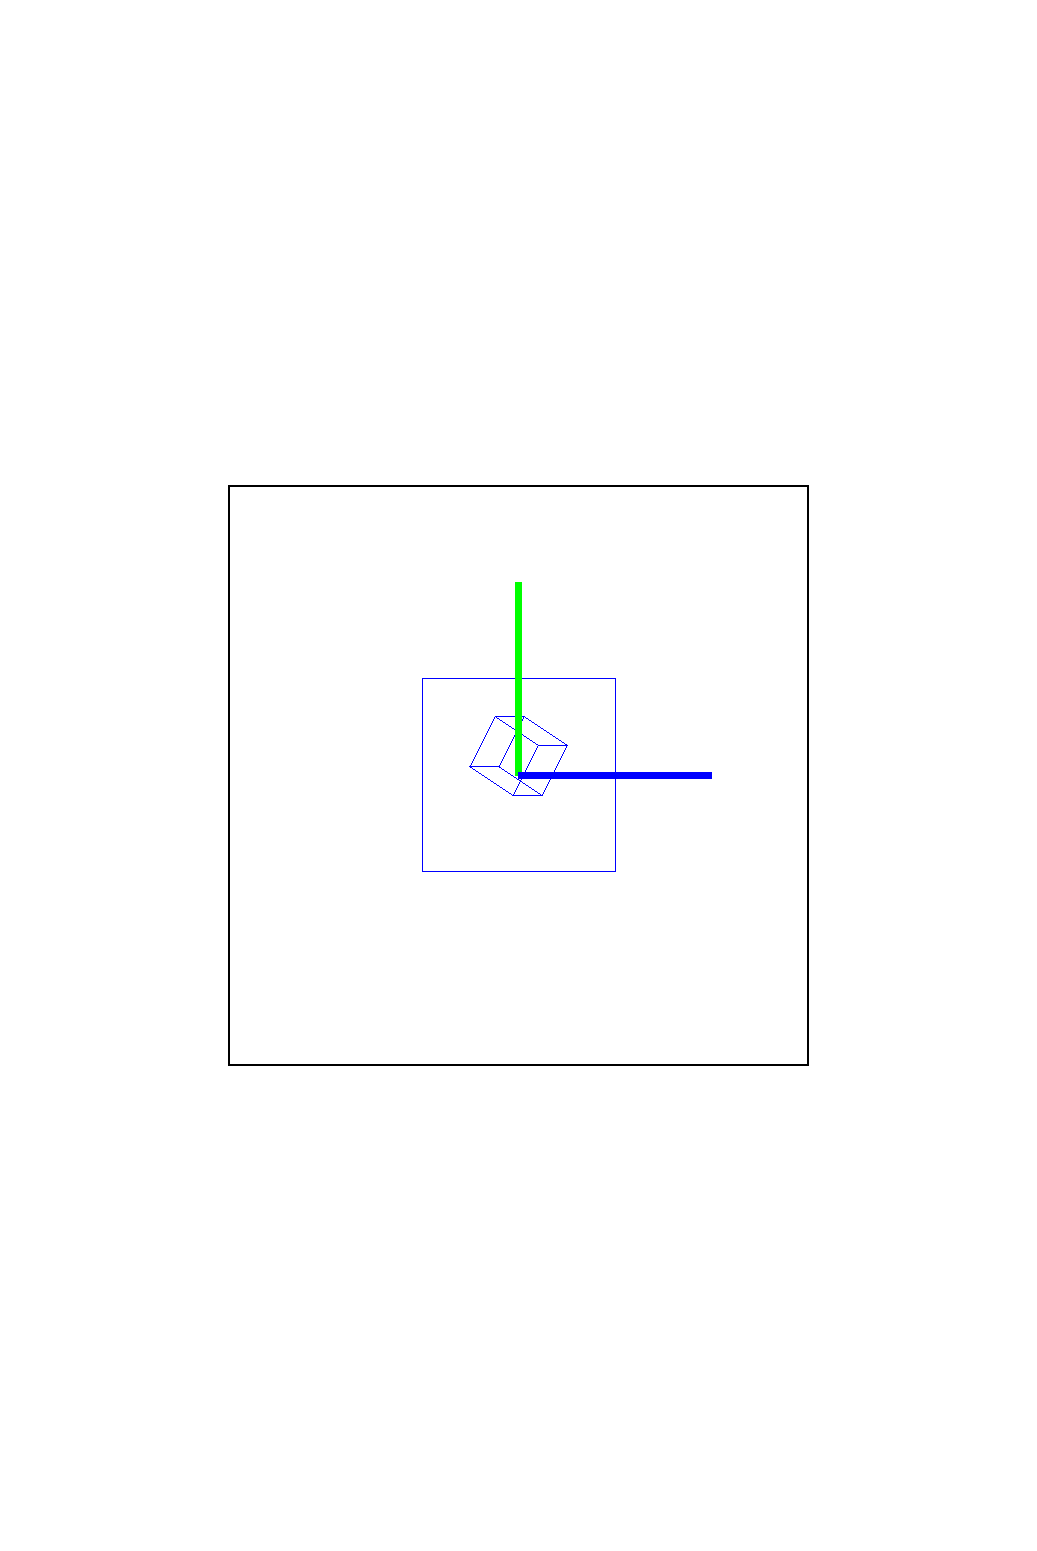
\includegraphics[bb=155 280 450 570,origin=c,scale=0.5,clip]{figure/box.eps}
  \end{center}
  \caption{The placement and rotation in the gsim4. The red, green, blue
  axes are x, y, z axes, respectively. The length of the axis line is 10
  cm.\label{box}} 
 \end{figure}

 {\tt /control/execute oglini.mac} is just for OpenGL visualization.
 The world is a box which has 3 paramters, full length of x, y, and z.
 Such parameters can be set with
 {\tt /GsimDetector/world/setParameters 30*cm 30*cm 30*cm}.
 Then, a new detector (box shaep), box, is created and placed at (0,0,0) with
 a rotation vector (0,0,0). Another box detector, box2, is created inside
 the ``box'' at (1*cm,1*cm,0) 
 with a rotation vector (30*deg 30*deg 0)
 with respect to the cordinate system of ``box''.
 
 Such rotation vector is the object rotation vector (not frame rotation
 vector). It means to rotate around x-axis with x component of the
 rotation vector, then rotate around y-axis with y component of the
 rotation vector, and finally rotate around z-axis with z component of
 the rotation vector.
 
 Actual volume creation, placement and
 rotation are perforemed after \\
 {\tt /GsimDetectorManager/update} is called.

 \subsubsection{Shapes}
 Several primitive shapes of detectors are prepared as follows.
 \begin{figure}[H]
  \begin{center}
   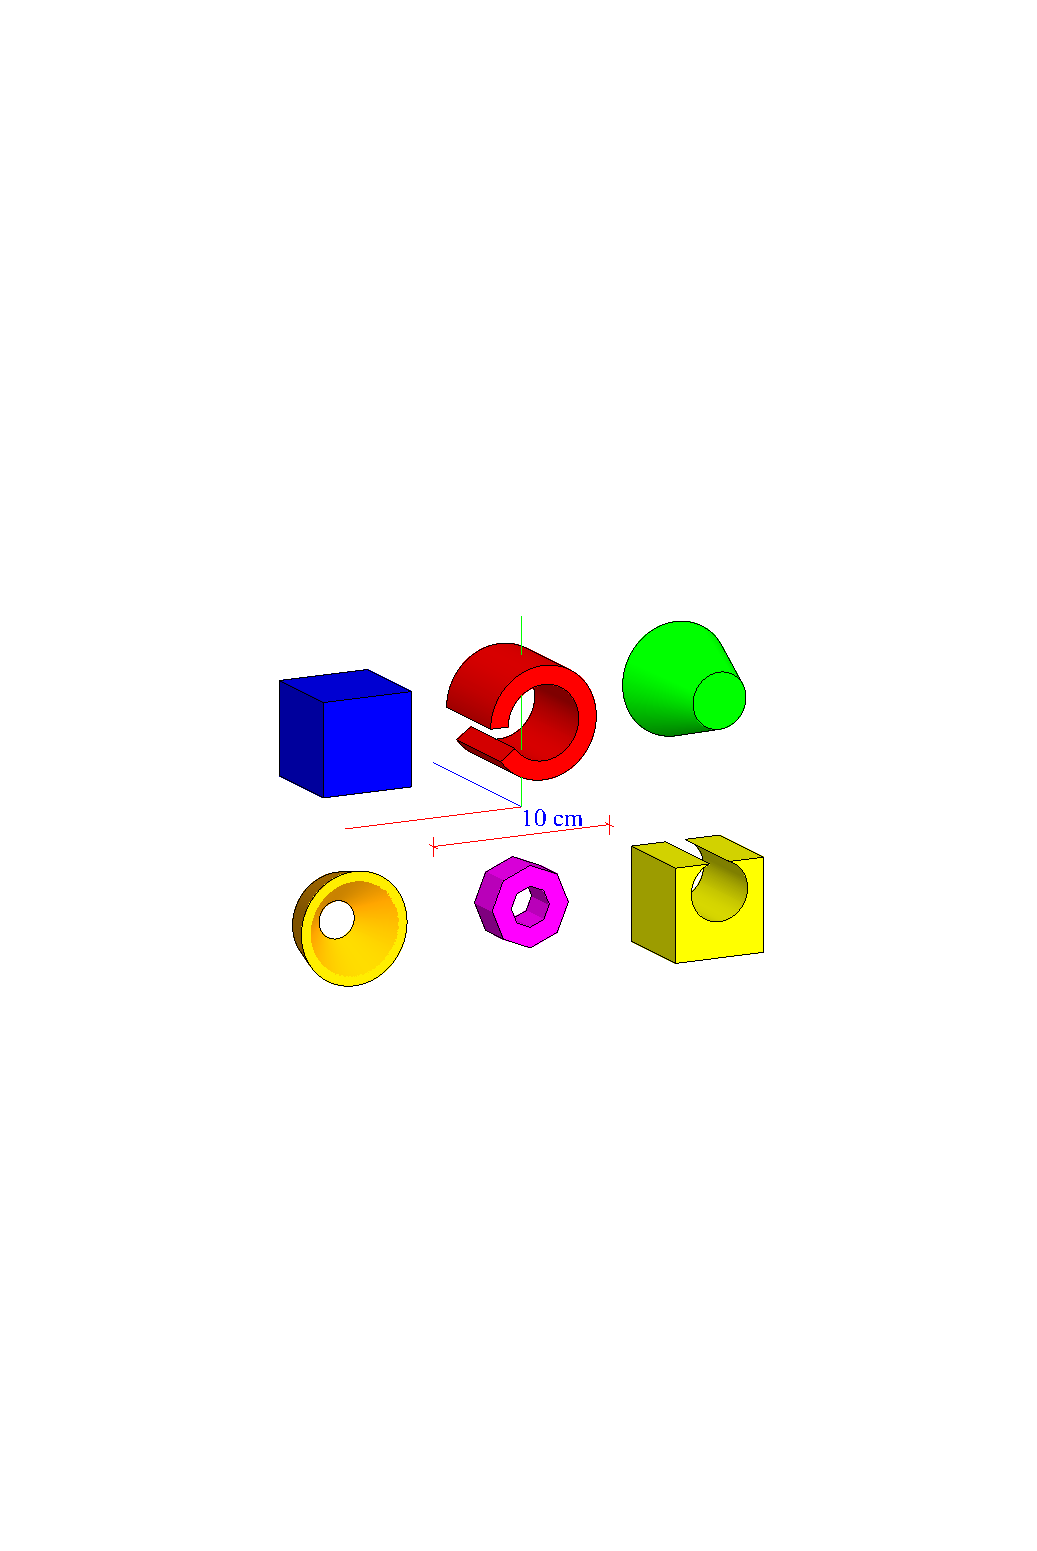
\includegraphics[bb=155 280 430 500,origin=c,scale=1.,clip]{figure/shape.eps}
  \end{center}
  \caption{The primitive shapes used in the gsim4. The red, green, blue
  axes are x, y, z axes, respectively.\label{shape}} 
 \end{figure}
 \begin{screen}\scriptsize
  \begin{verbatim}
/control/alias pos 5*cm

/GsimPhysicsListFactory/QGSP/buildAndRegister
/GsimPrimaryGeneratorActionFactory/GsimGeneralParticleSource/buildAndRegister gps
/GsimDetector/world/setOuterVisibility false

/GsimDetectorFactory/GsimBox/buildAndRegister box /world 2*{pos} {pos} 0
/GsimDetector/world/box/setParameters 5*cm 5*cm 5*cm
/GsimDetector/world/box/setOuterColor blue

/GsimDetectorFactory/GsimTube/buildAndRegister tube /world 0 {pos}  0
/GsimDetector/world/tube/setParameters 2*cm 3*cm 5*cm 0*rad 0.9*2.*pi*rad
/GsimDetector/world/tube/setOuterColor red

/GsimDetectorFactory/GsimCone/buildAndRegister cone /world -2*{pos} {pos} 0
/GsimDetector/world/cone/setParameters 1.5*cm 3*cm 5*cm
/GsimDetector/world/cone/setOuterColor green

/GsimDetectorFactory/GsimPolycone2/buildAndRegister pc2 /world 2*{pos} -{pos} 0
/GsimDetector/world/pc2/setParameters 0*deg 360*deg 20*mm 25*mm 30*mm 10*mm 25*mm
/GsimDetector/world/pc2/setOuterColor orange

/GsimDetectorFactory/GsimPolyhedra2/buildAndRegister ph2 /world 0 -{pos} 0
/GsimDetector/world/ph2/setParameters 0*deg 360*deg 8 20*mm 10*mm 20*mm
/GsimDetector/world/ph2/setOuterColor magenta

/GsimDetectorFactory/GsimBoxWithAHole/buildAndRegister boxh /world -2*{pos} -{pos} 0
/GsimDetector/world/boxh/setParameters 5*cm 5*cm 5*cm 0*cm 1*cm 1.6*cm
/GsimDetector/world/boxh/setOuterColor yellow

/GsimEventAction/setVisualizationMode 1
/control/execute oglsini.mac
#/control/execute dawnini.mac

/vis/viewer/set/viewpointThetaPhi 150 30
/vis/viewer/set/style s
/vis/scene/add/axes 0 0 0 10 cm
/vis/scene/add/scale 10 cm x 1 0 0 manual 0 -1.5 0 cm
/GsimDetectorManager/update\end{verbatim}
 \end{screen}
  The commands correspondig to such basic shapes are as follows.
  The shape parameters can be set with
  {\tt /GsimDetector/world/setParameters} with parameters.
  The number of such paramaeters must be the same as that required for
  the corresponding shape.
 \begin{itemize}
  \item /GsimDetectorFactory/GsimDetector/buildAndRegister\\
	This detector has no physical volume but just has logical
	structure, which can be used for grouping subdetectors.
	The number of dimensional parameters is 0.
  \item /GsimDetectorFactory/GsimBox/buildAndRegister\\
	The box shape.
	The number of dimensional parameters is 3.\\
	full length in x\\
	full length in y\\
	full length in z
  \item /GsimDetectorFactory/GsimBoxWithAHole/buildAndRegister\\
	The box shape with a hole inside.
	The number of dimensional parameters is 6.\\
	full length in x for the box\\
	full length in y for the box\\
	full length in z for the box\\
	x position of the center of the circle\\
	y position of the center of the circle\\
	radius of the circle
  \item /GsimDetectorFactory/GsimCone/buildAndRegister\\
	The cone shape.
	The number of dimensional parameters is 3.\\
	inner radius\\
	outer radius\\
	full length in z
  \item /GsimDetectorFactory/GsimPolycone2/buildAndRegister\\
	The polycone shape with 2 circler plains.
	The number of dimensional parameters is 7.\\
	start of the phi angle.\\
	opening ange for the phi\\
	full length in z\\
	inner radius for smaller z\\
	outer radius for smaller z\\
	inner radius for larger z\\
	outer radius for larger z
  \item /GsimDetectorFactory/GsimPolyhedra2/buildAndRegister\\
	The polyhedra shape with 2 rectangular plains.
	The number of dimensional parameters is 6.
	start of the phi angle.\\
	opening ange for the phi\\
	number of sides\\
	full length in z\\
	inner radius\\
	outer radius
  \item /GsimDetectorFactory/GsimTrap/buildAndRegister\\
	The trapezoidal shape.
	The number of dimensional parameters is 11.\\
	full length in z\\
	polar angle of the line joining the centres of the z faces\\
	azimuthal angle of the line joing the centre of the z faces\\
	full length along y on the plain of smaller z\\
	full length along x of the side at smaller y on the plain of smaller z\\
	full length along x of the side at larger y on the plain of smaller z\\
	angle of line joining the centres of the y sides w.r.t. the y
	axis on the plain of smaller z\\
	full length along y on the plain of larger z\\
	full length along x of the side at smaller y on the plain of larger z\\
	full length along x of the side at larger y on the plain of larger z\\
	angle of line joining the centres of the y sides w.r.t. the y
	axis on the plain of larger z
  \item /GsimDetectorFactory/GsimTube/buildAndRegister\\
	The tube shape.
	The number of dimensional parameters is 5.\\
	inner radius\\
	outer radius\\
	full length in z\\
	start of the phi angle.\\
	opening ange for the phi
 \end{itemize}
 \subsubsection{Volume material}
 Most outer volume for the detector can be modified. New material is
 assigned as follows.
 \begin{screen}
  \begin{verbatim}
/GsimDetector/world/box/setOuterMaterial G4_Fe\end{verbatim}
 \end{screen}
  All defined materials can be used including materials defined in
  G4NistMaterialBuilder, which are shown in Appendix.~\ref{app:mat}. 
 
 \subsubsection{Magnetic field}
 Magnetic field can be applied as follows.
 \begin{screen}
  \begin{verbatim}
/GsimDetector/world/box/setThisMagneticField 2*T 0 0\end{verbatim}
 \end{screen}
 The arguments means x, y, and z components of the magnetic field.
 
 %\subsubsection{Clone}
 % clone
 
 \subsection{Sensitivity}
 The detector sensitivity can be applied as follows.
  \begin{screen}
   \begin{verbatim}
/GsimDetector/world/e391/tube/setSensitiveDetectorWithName tube 0\end{verbatim}
  \end{screen}
  Here, most outer volume for the tube  get sensitivity  with module ID,
  0. Its SDname is tube.

 \subsection{Data storage}
 The data stored event by event are
 track information, hits information, and, digi information.
 Hits corresponds to all the steps with energy deposition.
 Digi corresponds to the sum of the hits per sensitive detector
 channnel. To store data or not can be controlled as follows.
 The hits information may become very huge, so it is not stored by
 default. Some fast simulation require hits information. Other data
 are stored by default.
 \begin{screen}
   \begin{verbatim}
   /GsimTrackingAction/setBriefTrackStore false
   /GsimDetector/world/e14/cv/setHitsStore true
   /GsimDetector/world/setThisAndDaughterHitsStore true
   /GsimDetector/world/e14/cv/setDigiStore true
  /GsimDetector/world/setThisAndDaughterDigiStore true\end{verbatim}
  \end{screen}
  
  Some commands to control the data storage are as follows.
  \begin{itemize}
   \item {\tt /GsimTrackingAction/setForceStorePrimary true}\\
	 Store primary information even if setBriefTrackStore is false.
   \item {\tt /GsimTrackingAction/setTrackHistory true}\\
	 Track history is filled or not.
   \item {\tt /GsimTrackingAction/addPIDToMonitor pid}\\
	 This pid is also monitored for the brief track.
   \item {\tt /GsimTrackingAction/clearPIDToMonitor}\\
	 Such monitor is canceled.
   \item {\tt /GsimTrackingAction/addPIDToTrigger pid}\\
	 If particles with the pid are generated,
	 the event is triggered for storage.
   \item {\tt /GsimTrackingAction/clearPIDToTrigger}\\
	 Such trigger is canceled.
   \item {\tt /GsimTrackingAction/addPIDToKill pid}\\
	 If a track with the pid is generated,
	 the track is killed immediately. The information of the track
	 is stored in the GsimGenParticleData if the pid is added for 
	 the monitoring.
   \item {\tt /GsimTrackingAction/clearPIDToKill}\\
	 Clear such pids to be killed.
   \item {\tt /GsimTrackingAction/setStoreAllTracks true}\\
	 All the tracks are sotred in GsimGenParticleData.
   \item {\tt /GsimEventAction/setSkipEmptyData false}\\
	 Skip if no data is filled in the sensitive detectors.
  \end{itemize}
  
 \subsection{Fast simulation}
 There are five kinds of fast simulation.
 One and two are to set fast simulation level at detector,
 third is to set
 online threshold at detector, and fourth is to use 
 ordering of  track stacking, and fifth is   
 to trigger with the end point of the primary track.
  \subsubsection{Fast simulation level at detector}
  Fast simulations can be done by assigning a fast simulation level to
  detectors as follows.
  \begin{screen}
   \begin{verbatim}
   /GsimDetector/world/e391/tube/setFastSimulationLevel 5\end{verbatim}
  \end{screen}
  It effects all detectors inside the detector.
  The meaning of the fast simulation levels are
  \begin{itemize}
   \item setFastSimulationLevel 6\\
	 This level is used for E14/E391 fast simulation.
	 Some unsensitive volumes are changed to be sensitive and some
	 support-structure voluems are moved to far upstream and become
	 invisible. 
	 Particles are stopped at the volume surface of the
	 detector. Such particle is treated as a hit, so
	 ``setHitsStore true'' is probably used together.
   \item setFastSimulationLevel 5\\
	 Particles are stopped at the volume surface of the
	 detector. Such particle is treated as a hit, so
	 ``setHitsStore true'' is probably used together.
   \item setFastSimulationLevel 4\\
	 Particles are stopped at one step inside the volume of the
	 detector.
   \item setFastSimulationLevel 3\\
	 Stop particles generated through ``conv'', ``eBrem'', and,
	 ''annihil''. (Stop shower-origin particles.)
   \item setFastSimulationLevel 2\\
	 Postpone a track process if the track pass
	 the boundary of brief detector.
  \end{itemize}
   \subsubsection{Online threshold at detector}
   The detecor online veto threshold is emulated.
   If the energy deposition at the sensitive detector exceeds the
   threshod, the event will be aborted immediately.
   \begin{screen}
   \begin{verbatim}
   /GsimSensitiveDetector/FBAR/setOnlineVetoThreshold 0.05*GeV\end{verbatim}
  \end{screen}
   \subsubsection{Stacking ordering}
   All the tracks are once stored in a stack, then which track in the
   stack will be processed first is decided with the stacking ordering.
   \begin{screen}
    \begin{verbatim}
    /GsimStackingAction/setBriefDtectorOrder BHCV CV BCV CC04\cdots\end{verbatim}
   \end{screen}
   \subsubsection{Trigger with the end point of the primary track.}
   This set the trigger z region for the the end point of the primary
   track. 
   If the end point of the primary track is located outside the
   region, the event will be aborted immediately.
   \begin{screen}
    \begin{verbatim}
    /GsimStackingAction/triggerPrimaryEndZ -10*m 10*m\cdots\end{verbatim}
   \end{screen}
   
  \subsection{Visualization}
  Some visualization control.
  \begin{itemize}
   \item {\tt /GsimEventAction/setVisualizationMode 1}\\
	 Tracks are displayd if some event display is prepared.
   \item {\tt /GsimEventAction/setAccumulationNumber num}\\
	 Set number of events overplayed in some event display.
   \item {\tt /GsimSteppingAction/setParticleColor pid colorName}\\
	 Set color of tracks.
  \end{itemize}
  
  \subsection{Debug}
  \begin{itemize}
   \item {\tt /GsimTrackingAction/setTrackDump true}\\
	 Dump of all tracks.
   \item {\tt /GsimEventAction/setVerboseLevel 0..4}
	 \begin{itemize}
	  \item 0 : verbosity off\\
	  \item 1 : error\\
	  \item 2 : warning\\
	  \item 3 : info\\
	  \item 4 : debug\\
	 \end{itemize}
   \item {\tt /GsimEventAction/setDumpMode 0..3}
	 \begin{itemize}
	  \item 0 : no dump
	  \item 1 : dump first 10 events
	  \item 2 : dump all events
	  \item 3 : dump all events with timing
	 \end{itemize}
   \item {\tt /GsimEventAction/writeDictionary true}\\
	 Write a text-file dicitonary.
  \end{itemize}
 \section{Optical photon Simulation}
 {\tt
 \$E14\_TOP\_DIR/examples/gsim4test/test15.mac}\\
 
 {\tt
 \$E14\_TOP\_DIR/examples/gsim4test/test16.mac}
 
 \section{E14 Fast Simulation}
 There are three steps.
 \begin{enumerate}
  \item Fast simulation (particle decay and transportation)\\
	The same geometery as the full
	simulation is used.\
	The gsim4test with the fastSimulationLevel, 6, is used.
  \item Detector fast simulation\\
	Some smearing on the energy and angle is applied.
	Fusion in CsI is treated. Veto weights are calculated according
	to the models of the  detector ineffieicnecy. Finally events are
	classified with the number of clusters in the CsI.
  \item Two gamma analysis is applied for the $K_L\to\pi^0\nu\nu$
	analysis.
 \end{enumerate}

 
 \section{Developement}
 \subsection{Adding Branch or Histogram}
 Some member functions of GsimPersistencyManager can be used. The
 GsimPersistencyManager class is a singleton class, which can be used
 at anywhere with ``GsimPersistencyManager::getPersistencyManager()''.
 \begin{verbatim}
void GsimPersistencyManager::setBranchOf(std::string treeName,
                   std::string title,
                   std::string className,
                   void* address);

void GsimPersistencyManager::setBranchOf(std::string treeName,
                   std::string title,
                   void* address,
                   std::string format);
 \end{verbatim}
 The ``treeName'' can be ``runTree'',``eventTree'',$\cdots$. ``format''
 can be ``num/I'', ``val/D'' as used in ``ROOT''.
 \begin{verbatim}	
TH1D* GsimPersistencyManager::createHistogram(char* name,char* title,
                        int nbin,double xmin,double xmax);
void  GsimPersistencyManager::fillHistogram(char* name,double value);

TH2D* GsimPersistencyManager::createHistogram(char* name,char* title,
                        int nbinx,double xmin,double xmax,
                        int nbiny,double ymin,double ymax);
void  fillHistogram(char* name,double xvalue,double yvalue);
 \end{verbatim}
 The useage is as follows. You can find some example in\\
 \$E14TOPDIR/sources/sim/gsim4/GsimE14Spectrum/src/GsimE14HalonSpectrum.cc.
 \begin{verbatim}
GsimPersistencyManager::getPersistencyManager()
    ->createHistogram("hE14HalonMome","hE14HalonMome [GeV/c]",
                      150,0,15);
GsimPersistencyManager::getPersistencyManager()
    ->fillHistogram("hE14Mome",p.mag());
 \end{verbatim}






 \subsection{Your own detector class}
 \section{Analysis}

 
 % \section{Command reference}
%  \subsubsection{GsimDetectorFactory}

 
%  A detector has a name and full path.
%  The world has a name,'world' and full path,'/world'.
%  If a detector with its name of `A` is plaeed in the world,
%  the detector has a name, 'A' and full path, '/world/A'.
%  The detector placement is treated as a directory tree.

 
%  The placement inside the same mother volume at the creation can
%  be done /GsimDetector/ commands afterwords. Its relation to the mother
%  detector can't be changed.
 
%  Actual creation, placement and
%  rotation are perforemed after /GsimDetectorManager/update.
 
 
 
%  The dimenstion of a detector are set by /GsimDetector/
%  commands.

%  The translation vector means to place the detector center to
%  the translation vector from the center of the mother detector.
%  The rotation vector is the object rotation vector (not frame rotation
%  vector). It means to rotate around x-axis with x component of the
%  rotation vector, then rotate around y-axis with y component of the
%  rotation vector, and finally rotate around z-axis with z component of
%  the rotation vector.

%  The following arguments are treated.
%  \begin{itemize}
%   \item The number of argments is 8.\\
% 	.../buildAndRegister\\
% 	this detector name\\
% 	mother full path\\
% 	translation x\\
% 	translation y\\
% 	translation z\\
% 	rotation x\\
% 	rotation y\\
% 	rotation z\\
%   \item The number of argments is 7.\\
% 	.../buildAndRegister\\
% 	this detector name\\
% 	translation x\\
% 	translation y\\
% 	translation z\\
% 	rotation x\\
% 	rotation y\\
% 	rotation z\\
% 	Here, the mother full path is /world.
%   \item The number of argments is 5.\\
% 	.../buildAndRegister\\
% 	this detector name\\
% 	mother full path\\
% 	translation x\\
% 	translation y\\
% 	translation z\\
% 	No rotation is applied.
%   \item The number of argments is 4.\\
% 	.../buildAndRegister\\
% 	this detector name\\
% 	translation x\\
% 	translation y\\
% 	translation z\\
% 	The mother full path is /world and no rotation is applied.
%   \item The number of argments is 2.\\
% 	.../buildAndRegister\\
% 	this detector name\\
% 	mother full path\\
% 	The translation is set to the origin and no rotation is applied.
%   \item The number of argments is 1.\\
% 	.../buildAndRegister\\
% 	this detector name\\
% 	The mother full path is /world, the translation is set to the
% 	origin and no rotation is applied. 
%  \end{itemize}

%  \subsection{Detector}
%  \begin{itemize}
%   \item /GsimDetector/setTranslationVector\\
% 	x\\
% 	y\\
% 	z\\
% 	Set the translation vector for the placement.
% 	Place the detector cetner at the the translation vector
% 	from the center of the mother detector.
%   \item /GsimDetector/setLocalCenterVector\\
% 	x\\
% 	y\\
% 	z\\
% 	Set the detector center from the default cetner, which is
% 	defined by geant4.
%   \item /GsimDetector/setRotationVector\\
% 	rotation around x-axis\\
% 	rotation around y-axis\\
% 	rotation around z-axis\\
% 	Set the detector rotation (object rotation).
% 	The order is rotation around x, y, and z.

%   \item /GsimDetector/cloneDetector\\
% 	translation x\\
% 	translation y\\
% 	translation z\\
% 	rotation around x axis\\
% 	rotation around y axis\\
% 	rotation around z axis\\
% 	channel number to be assinged
%   \item /GsimDetector/clearThisClone\\
	
%   \item /GsimDetector/setThisAndDaughterBriefName\\

	
%   \item /GsimDetector/setOuterMaterial\\
%   \item /GsimDetector/setOuterColor\\
%   \item /GsimDetector/setOuterVisibility\\
%   \item /GsimDetector/setThisAndDaughterOuterVisibility\\
%   \item /GsimDetector/setParameters\\

	
%   \item /GsimDetector/setThisMagneticField\\
%   \item /GsimDetector/setThisAndDaughterMagneticField\\
	
  

%   \item /GsimDetector/setSensitiveVolume\\
%   \item /GsimDetector/setSensitiveDetector\\
%   \item /GsimDetector/setSensitiveDetectorWithName\\

  

%   \item /GsimDetector/setHitsStore\\
%   \item /GsimDetector/setHitsStoreDaughters\\
%   \item /GsimDetector/setDigiStore\\
%   \item /GsimDetector/setDigiStoreDaughters\\

%   \item /GsimDetector/setFastSimulationLevel\\
	
%   \item /GsimDetector/setThisUserStepMax\\
%   \item /GsimDetector/setThisUserTrackMax\\
%   \item /GsimDetector/setThisUserTimeMax\\
%   \item /GsimDetector/setThisUserEkinMin\\
%   \item /GsimDetector/setThisUserRangeMin\\
%   \item /GsimDetector/resetThisUserLimits\\
%   \item /GsimDetector/setThisAndDaughterUserStepMax\\
%   \item /GsimDetector/setThisAndDaughterUserTrackMax\\
%   \item /GsimDetector/setThisAndDaughterUserTimeMax\\
%   \item /GsimDetector/setThisAndDaughterUserEkinMin\\
%   \item /GsimDetector/setThisAndDaughterUserRangeMin\\
%   \item /GsimDetector/resetThisAndDaughterUserLimits\\
%   \item /GsimDetector/setUserInputs\\
  
%   \item /GsimDetector/setThisAsARootRegion\\
  
  
  
  
%   \item /GsimDetector/print\\
%   \item /GsimDetector/update\\
%  \end{itemize}
 \section{Description about the stored data structure}
 The Data is stored in ROOT TTree in TFile.
 \begin{screen}
  {\tt root\return\\}
  {\tt std::string dir=std::getenv("E14\_TOP\_DIR");}\\
  {\tt dir+="/lib/so/libGsimData.so");}\\
  {\tt gSystem->Load(dir.c\_str());}\\
  {\tt TFile* tf = new TFile(''tmp.root'');}
  {\tt tf->ls();}
{\small
TFile**         tmp.root        \\
 TFile*         tmp.root        \\
  KEY: TTree    detectorTree00;1        detectorTree00\\
  KEY: TTree    physicalVolumeTree00;1  physicalVolumeTree00\\
  KEY: TTree    processTree00;1 processTree00\\
  KEY: TTree    eventTree00;1   eventTree00\\
  KEY: TTree    eventSeedTree00;1       eventSeedTree00\\
  KEY: TTree    commandTree;1   commandTree\\
  KEY: TTree    runTree;1       runTree\\
  }
 \end{screen}

 \begin{figure}[H]
  \begin{center}
   \includegraphics[scale=0.5]{xwd/top.eps}
  \end{center}
  \caption{Top.}
 \end{figure}
 
 \begin{itemize}
  \item commandTree\\
	Each command typed or in macro file.
  \item runTree
  \item detectorTree00
  \item physicalVolumeTree00
  \item processTree00
  \item eventTree00
  \item eventSeedTree00
 \end{itemize}

 \subsection{commandTree}
 Each command typed or executed in macro file is sotred.
 \begin{figure}[H]
  \begin{center}
   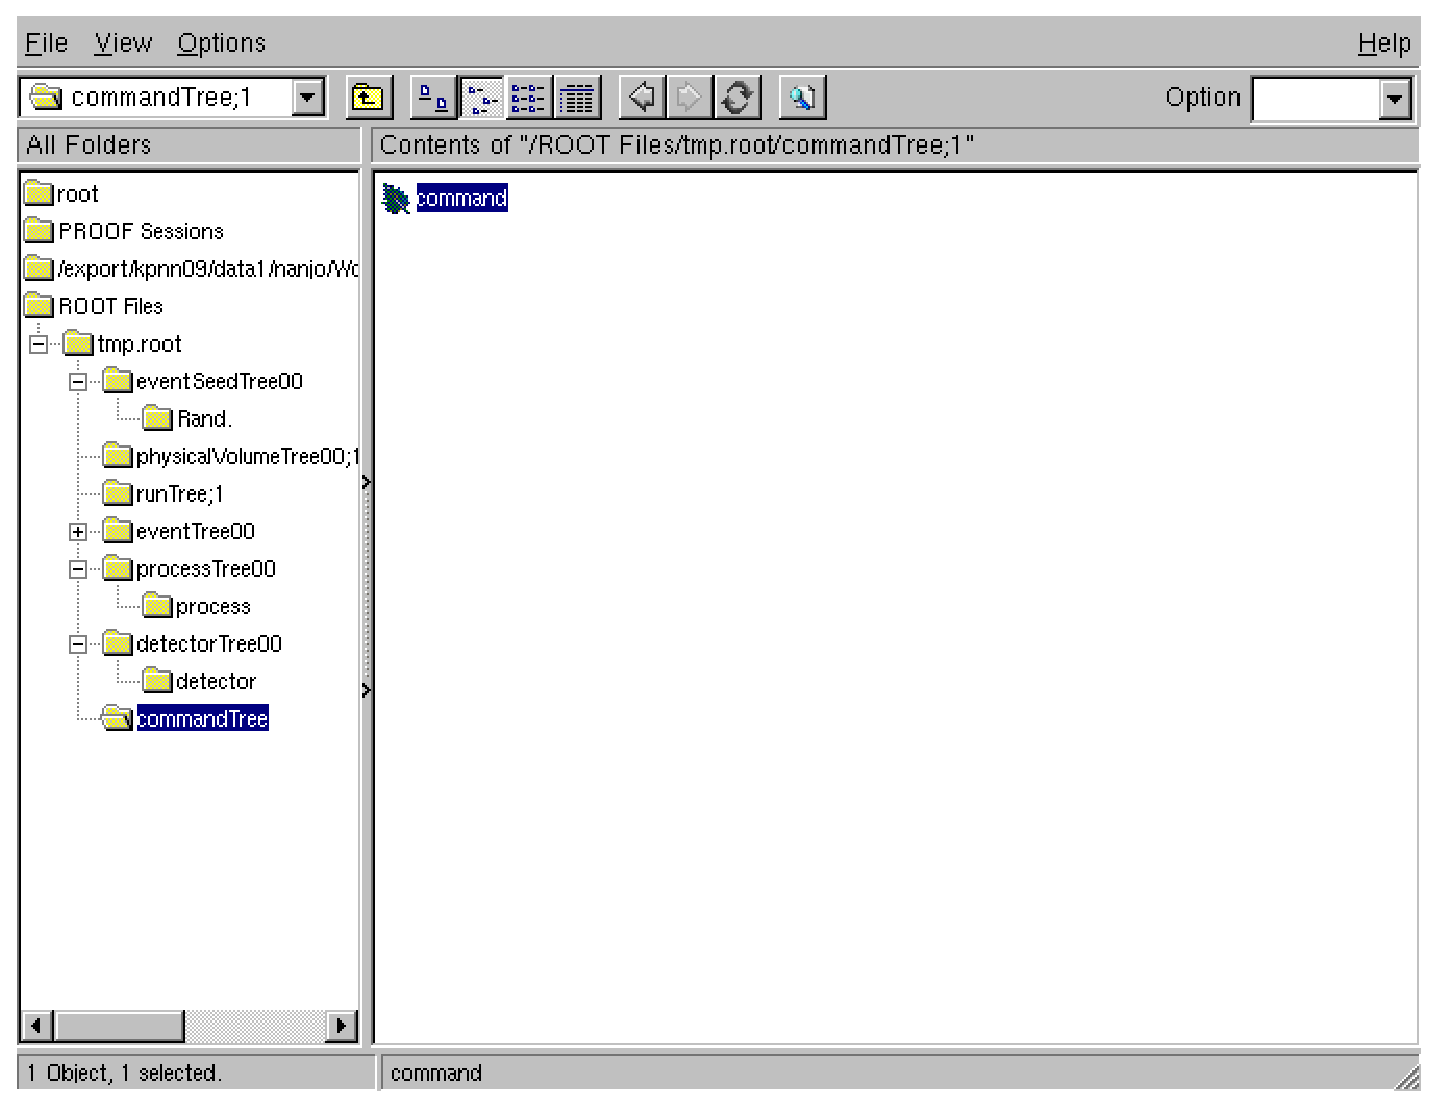
\includegraphics[scale=0.5]{xwd/cm.eps}
  \end{center}
  \caption{commandTree.}
 \end{figure}

  \subsection{runTree}
  \begin{figure}[H]
   \begin{center}
    \includegraphics[scale=0.5]{xwd/rn.eps}
   \end{center}
   \caption{runTree.}
  \end{figure}

  \begin{itemize}
   \item runNumber
   \item runID
   \item nEventsRequested
   \item nEventsProcessed
   \item nEventsStored
   \item version
  \end{itemize}

  \subsection{processTree}
  \begin{figure}[H]
   \begin{center}
    \includegraphics[scale=0.5]{xwd/pr.eps}
   \end{center}
   \caption{processTree}
  \end{figure}
  
  \begin{itemize}
   \item processID
   \item processName
  \end{itemize}

  \subsection{physicalVolumeTree}
   \begin{figure}[H]
   \begin{center}
    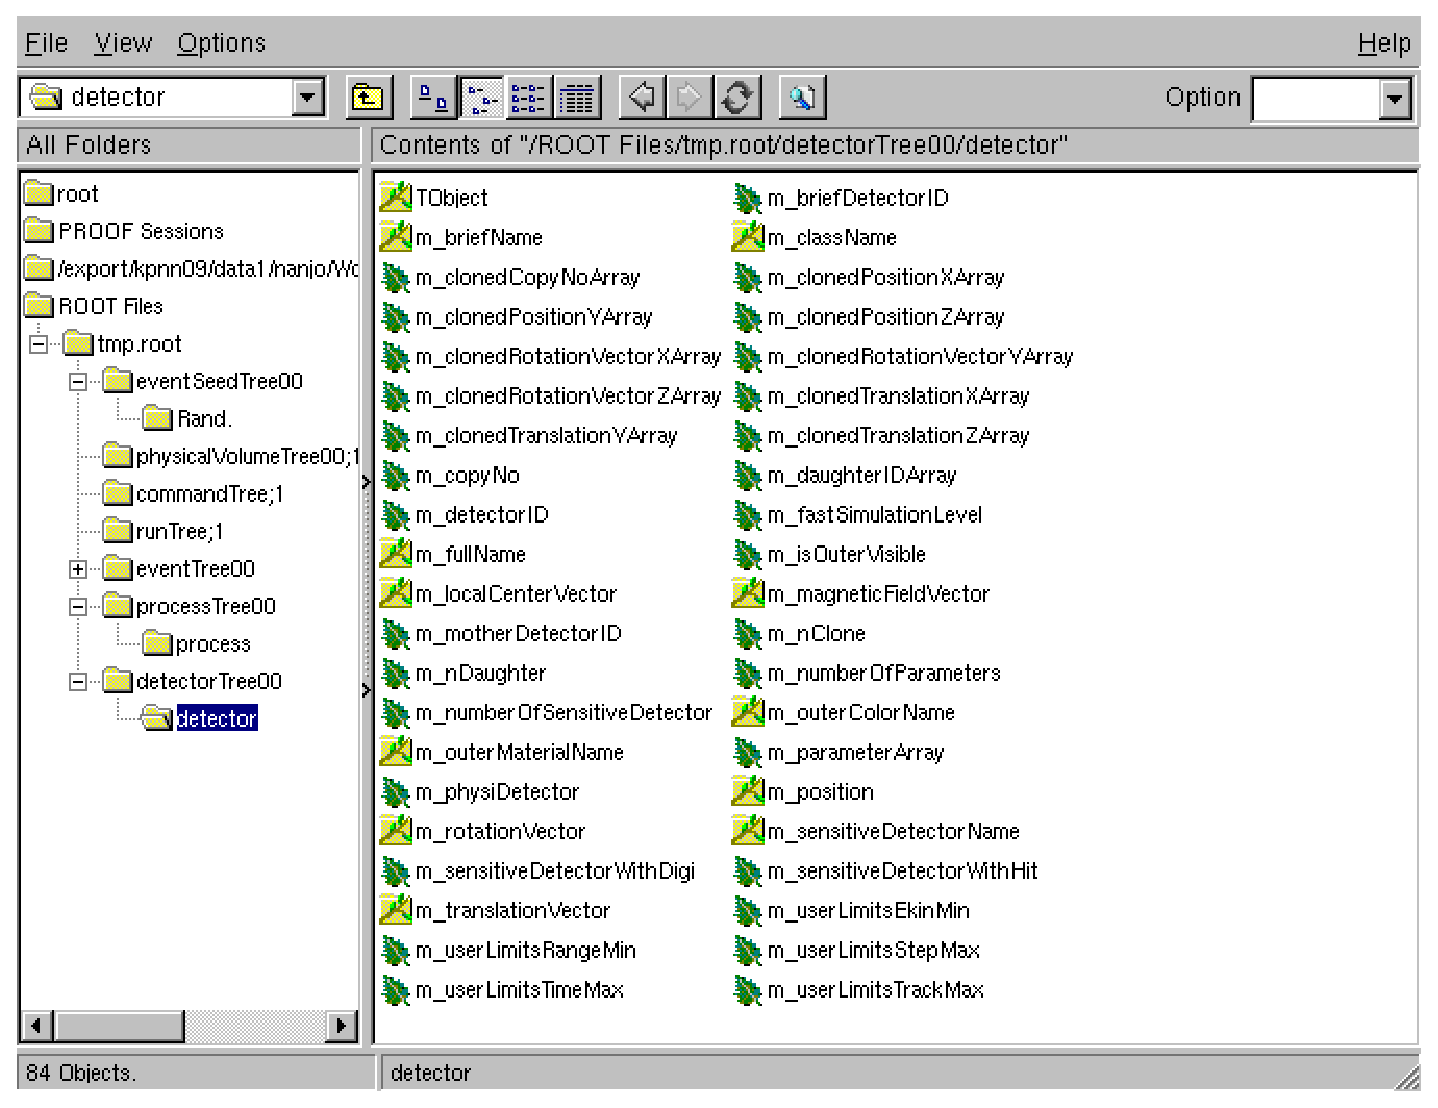
\includegraphics[scale=0.5]{xwd/de.eps}
   \end{center}
    \caption{pysicalVolumeTree.}
   \end{figure}

   \begin{itemize}
    \item pvName
    \item pvopyNo
    \item detID
    \item detFullName
    \item detBriefName
    \item sdFlag
    \item sdName
    \item sdID
    \item sdNch
    \item sdChID[sdNch]
    \item sdClIDl[sdNch]
   \end{itemize}
   
  \subsection{detectorTree}
  \begin{figure}[H]
   \begin{center}
    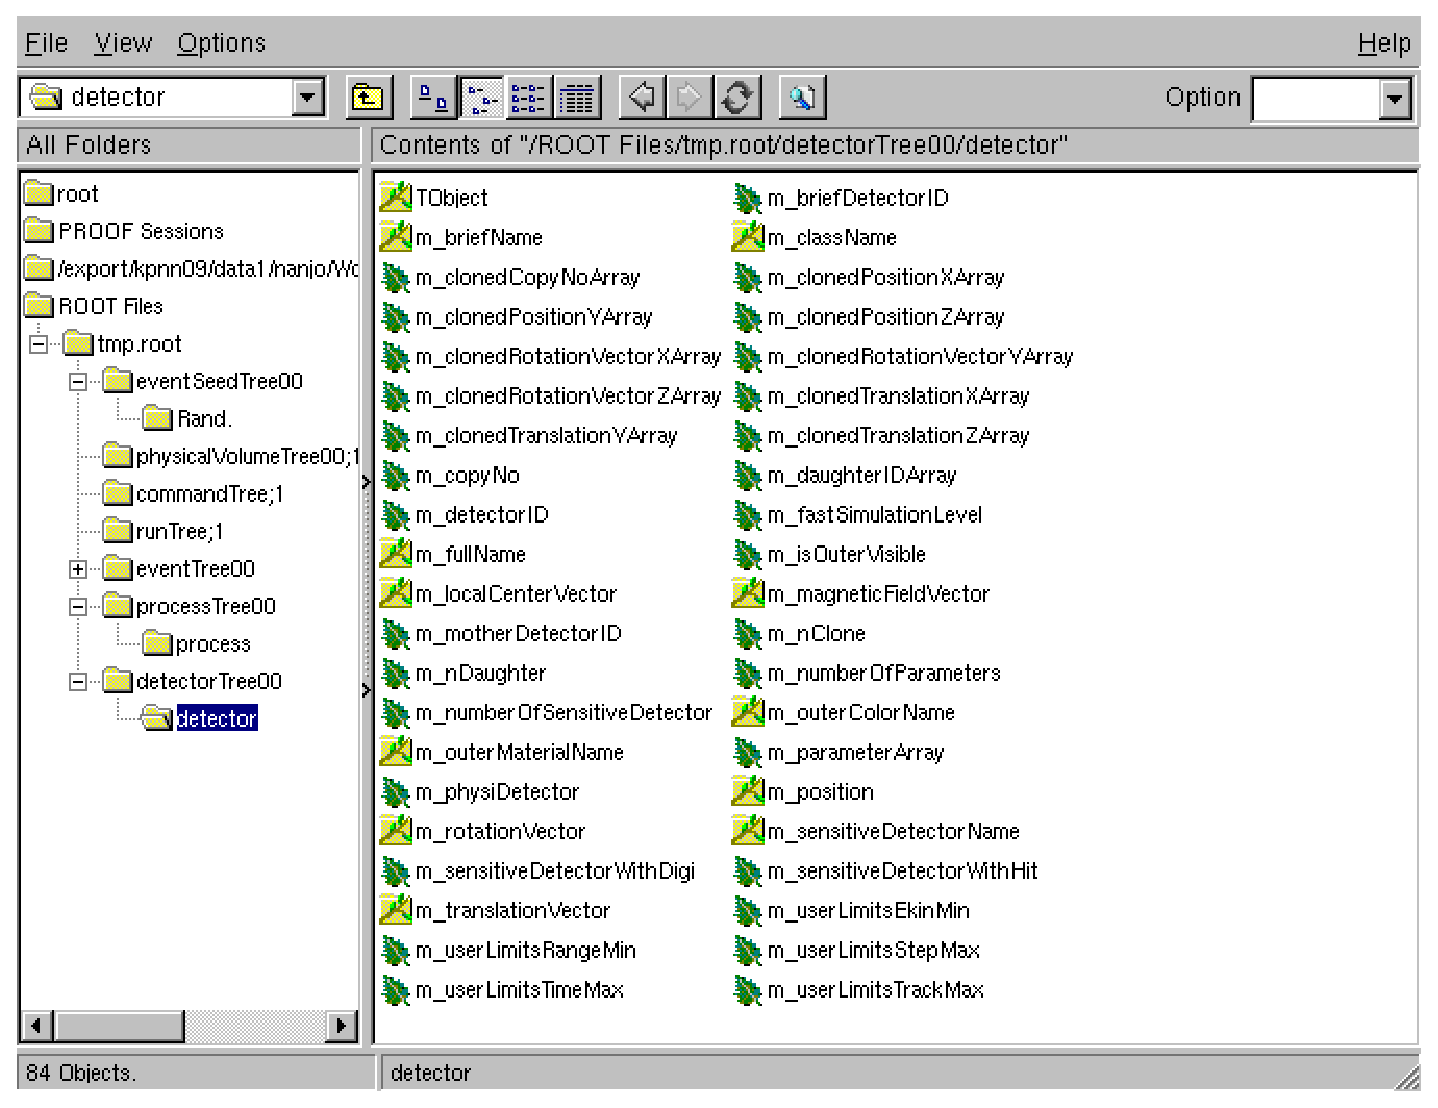
\includegraphics[scale=0.5]{xwd/de.eps}
   \end{center}
   \caption{detectorTree.}
  \end{figure}

  \subsection{eventSeedTree}
  \begin{figure}[H]
   \begin{center}
    \includegraphics[scale=0.5]{xwd/rn.eps}
   \end{center}
   \caption{eventSeedTree.}
  \end{figure}
  \begin{itemize}
   \item run\_number
   \item event\_number
   \item engineID
   \item seed[624]
   \item count
   \item version
  \end{itemize}
   
  \subsection{eventTree}
  Digi/hits information is stored in corresponding sensitive detector.
   \begin{figure}[H]
    \begin{center}
     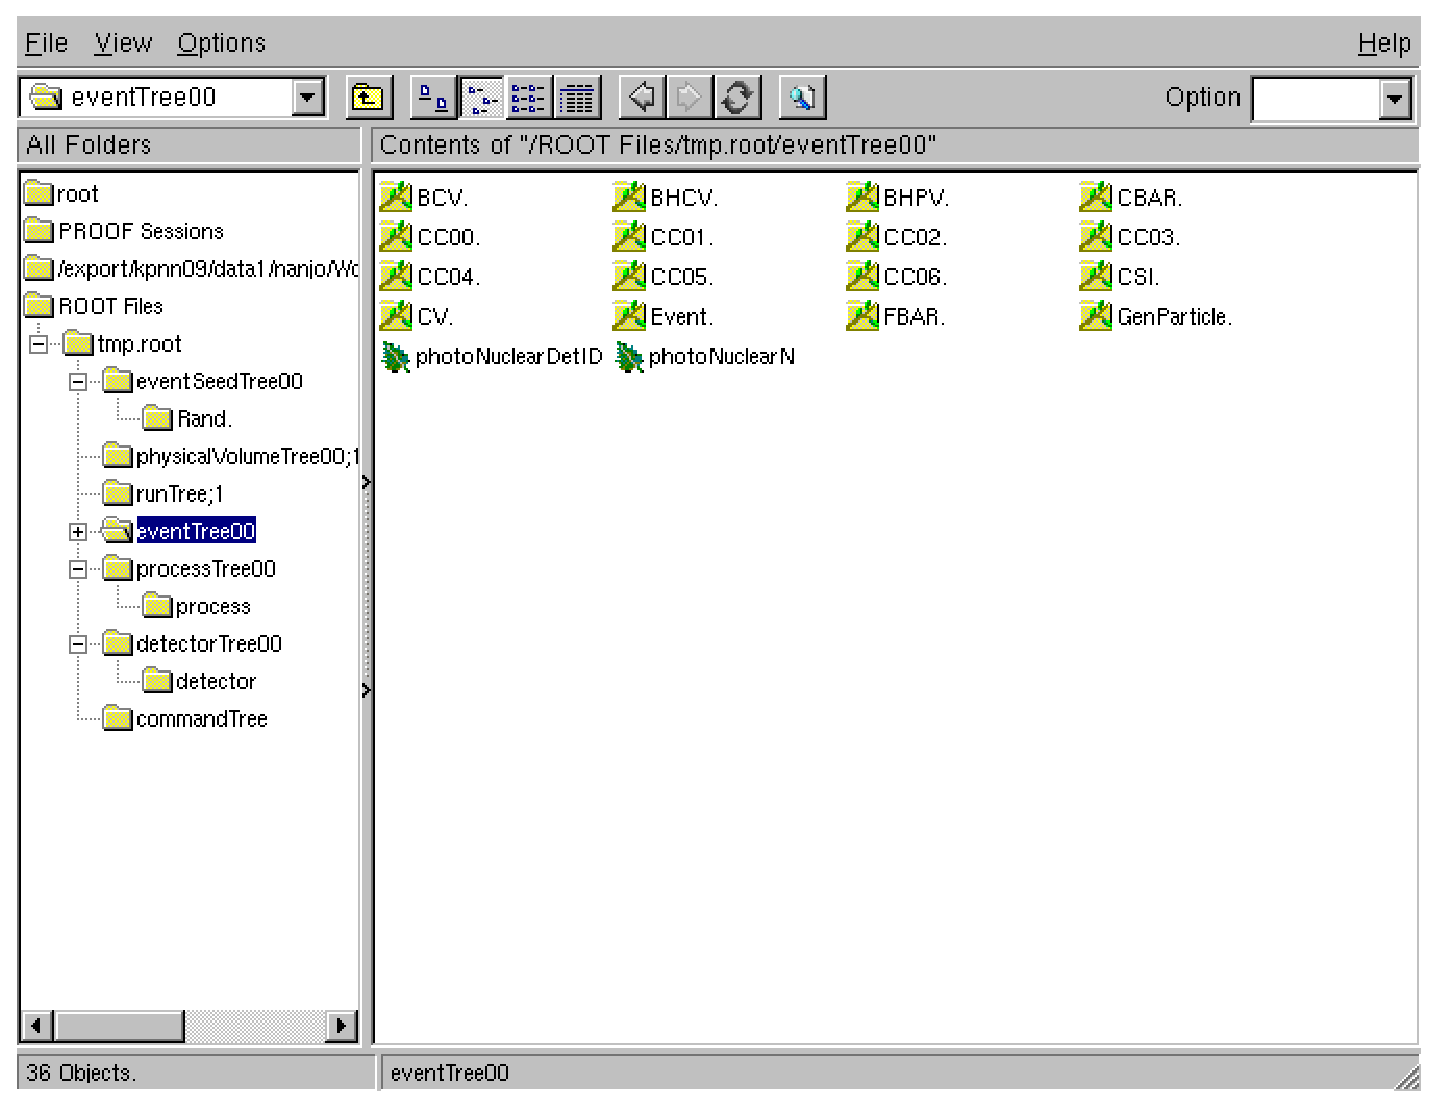
\includegraphics[scale=0.5]{xwd/et.eps}
    \end{center}
    \caption{eventTree.}
   \end{figure}

   \subsubsection{GenParticle}
   GenParticle is ROOT ``TClonesArray'' for GsimBriefTrack.
   \begin{figure}[H]
    \begin{center}
     \includegraphics[scale=0.5]{xwd/bt.eps}
    \end{center}
    \caption{briefTracks.}
   \end{figure}

   \begin{itemize}
    \item GenParticle.briefTracks\\
	  The TClonesArray for GsimTrackDaa.
    \item GenParticle.briefTracks.track\\
	  The track ID (assinged by Geant4). 
    \item GenParticle.briefTracks.mother\\
	  The track ID for the mother track, which is stored as breif tracks.
    \item GenParticle.briefTracks.pid\\
	  The particle ID.
    \item GenParticle.briefTracks.p\\
	  TVector3 momentum.
    \item GenParticle.briefTracks.ek\\
	  Kinetic energy.
    \item GenParticle.briefTracks.mass\\
	  Mass.
    \item GenParticle.briefTracks.time\\
	  The time the particle is created.
    \item GenParticle.briefTracks.v\\
	  The vertex position where the particle is created.
    \item GenParticle.briefTracks.mech\\
	  The id of the creation mechanism for the track.
    \item GenParticle.briefTracks.status\\
	  The track status.
    \item GenParticle.briefTracks.thisID\\
	  ID assigned by gsim4.
    \item GenParticle.briefTracks.history\\
	  The volume history.
    \item GenParticle.version\\
	  The version of this data structre.
   \end{itemize}

   \subsubsection{Sensitive detector}
   Digi, hits, etc are for each sensitive detector are stored.. 
   \begin{figure}[H]
    \begin{center}
     \includegraphics[scale=0.5]{xwd/cv.eps}
    \end{center}
    \caption{Sensitive detector, for example CV.}
   \end{figure}
    
    \begin{figure}[H]
     \begin{center}
      \includegraphics[scale=0.5]{xwd/digi.eps}
     \end{center}
     \caption{digi for example, CV.}
    \end{figure}

    \begin{itemize}
     \item CV.digi.detID\\
	   detector ID. 
     \item CV.digi.modID\\
	   module ID (channel assignment).
     \item CV.digi.energy\\
	   total energy deposition at the module.
     \item CV.digi.time\\
	   First hit timing (threshold/pileup effects are treated).
     \item CV.digi.thisID\\
	   ID for TClonesArray of GsimDigiData.
     \item CV.digi.status (stop+10*fastSimulationLevel)\\
	   fAlive:Continue the tracking\\
	   fStopButAlive:Invoke active rest physics processes and kill the current track afterward\\
	   fStopAndKill: Kill the current track\\
	   fKillTrackAndSecondaries: Kill the current track and also
	   associated secondaries.\\
	   fSuspend:Suspend the current track\\
	   fPostponeToNextEvent: Postpones the tracking of thecurrent
	   track to the next event. 
     \item CV.digi.track\\
	   Stored track ID
     \item CV.digi.mtimeEntry\\
	   Digi is created form bounch of hits along time. Suc hits are
	   stored in mtime. mtimeEntry point to that.
     \item CV.digi.mtimeSize\\
	   number of mtime entry.
    \end{itemize}

    \begin{figure}[H]
     \begin{center}
      \includegraphics[scale=0.5]{xwd/mtime.eps}
     \end{center}
     \caption{mtime.}
    \end{figure}

    \begin{itemize}
     \item CV.mtime.modID\\
	   module ID.
     \item CV.mtime.energy\\
	   multi hit time energy.
     \item CV.mtime.time\\
	   multi hit time.
    \end{itemize}
    
    \begin{figure}[H]
     \begin{center}
      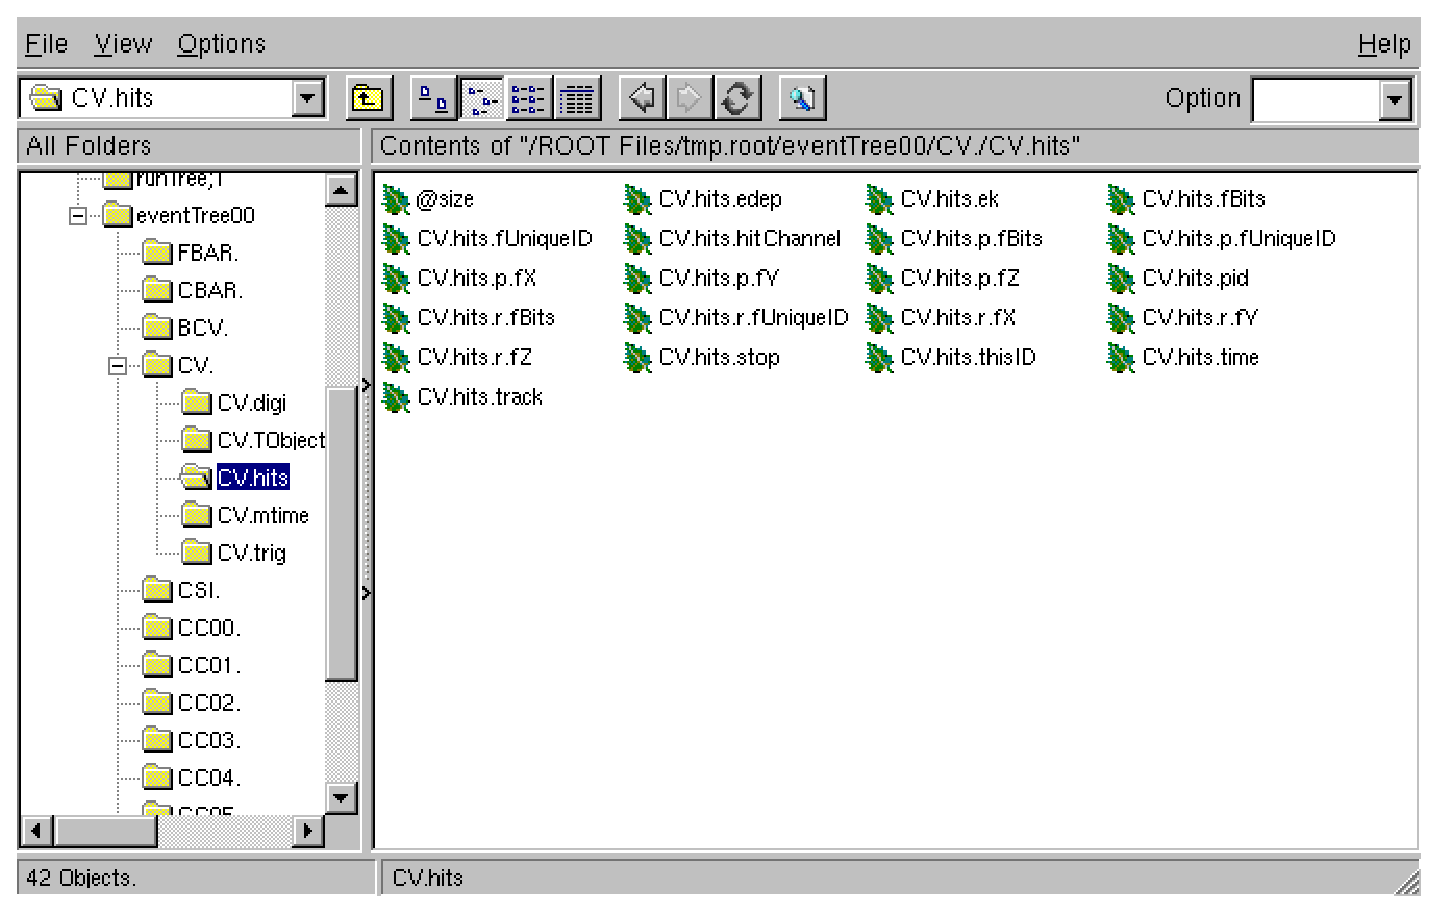
\includegraphics[scale=0.5]{xwd/hit.eps}
     \end{center}
     \caption{}
    \end{figure}

    \begin{itemize}
     \item CV.hits.thisID
     \item CV.hits.track\\
	   track ID
     \item CV.hits.stop\\
	   stop flag
     \item CV.hits.hitChannel\\
	   hit channel
     \item CV.hits.time\\
	   hit time
     \item CV.hits.edep\\
	   edep.
     \item CV.hits.pid\\
	   pid.
     \item CV.hits.r\\
	   position
     \item CV.hits.ek\\
	   kinetic energy
     \item CV.hits.p\\
	   momentum
    \end{itemize}
    
    
    \begin{figure}[H]
     \begin{center}
      \includegraphics[scale=0.5]{xwd/trig.eps}
     \end{center}
     \caption{trig.}
    \end{figure}
    
    \begin{itemize}
     \item CV.trig.modID\\
	   triggered moduleID
     \item CV.trig.energy\\
	   triggered module energy
     \item CV.trig.time\\
	   triggered time.
    \end{itemize}
    
 \newpage
 \appendix
 \section{Materials prepared in Geant4\label{app:mat}}
 \begin{verbatim}
  AddMaterial("G4_H" ,  8.37480e-5,  1,  19.2, 1, kStateGas);
  AddMaterial("G4_He",  1.66322e-4,  2,  41.8, 1, kStateGas);
  AddMaterial("G4_Li",  0.534     ,  3,  40. );
  AddMaterial("G4_Be",  1.848     ,  4,  63.7);
  AddMaterial("G4_B" ,  2.37      ,  5,  76. );
  AddMaterial("G4_C" ,  2.        ,  6,  81. );
  AddMaterial("G4_N" ,  1.16520e-3,  7,  82. , 1, kStateGas);
  AddMaterial("G4_O" ,  1.33151e-3,  8,  95. , 1, kStateGas);
  AddMaterial("G4_F" ,  1.58029e-3,  9, 115. , 1, kStateGas);
  AddMaterial("G4_Ne",  8.38505e-4, 10, 137. , 1, kStateGas);
  AddMaterial("G4_Na",  0.971     , 11, 149. );
  AddMaterial("G4_Mg",  1.74      , 12, 156. );
  AddMaterial("G4_Al",  2.699     , 13, 166. );
  AddMaterial("G4_Si",  2.33      , 14, 173. );
  AddMaterial("G4_P" ,  2.2       , 15, 173. );
  AddMaterial("G4_S" ,  2.0       , 16, 180. );
  AddMaterial("G4_Cl",  2.99473e-3, 17, 174. , 1, kStateGas);
  AddMaterial("G4_Ar",  1.66201e-3, 18, 188.0, 1, kStateGas);
  AddMaterial("G4_K" ,  0.862     , 19, 190. );
  AddMaterial("G4_Ca",  1.55      , 20, 191. );
  AddMaterial("G4_Sc",  2.989     , 21, 216. );
  AddMaterial("G4_Ti",  4.54      , 22, 233. );
  AddMaterial("G4_V" ,  6.11      , 23, 245. );
  AddMaterial("G4_Cr",  7.18      , 24, 257. );
  AddMaterial("G4_Mn",  7.44      , 25, 272. );
  AddMaterial("G4_Fe",  7.874     , 26, 286. );
  AddMaterial("G4_Co",  8.9       , 27, 297. );
  AddMaterial("G4_Ni",  8.902     , 28, 311. );
  AddMaterial("G4_Cu",  8.96      , 29, 322. );
  AddMaterial("G4_Zn",  7.133     , 30, 330. );
  AddMaterial("G4_Ga",  5.904     , 31, 334. );
  AddMaterial("G4_Ge",  5.323     , 32, 350. );
  AddMaterial("G4_As",  5.73      , 33, 347. );
  AddMaterial("G4_Se",  4.5       , 34, 348. );
  AddMaterial("G4_Br",  7.07210e-3, 35, 343. , 1, kStateGas);
  AddMaterial("G4_Kr",  3.47832e-3, 36, 352. , 1, kStateGas);
  AddMaterial("G4_Rb",  1.532     , 37, 363. );
  AddMaterial("G4_Sr",  2.54      , 38, 366. );
  AddMaterial("G4_Y" ,  4.469     , 39, 379. );
  AddMaterial("G4_Zr",  6.506     , 40, 393. );
  AddMaterial("G4_Nb",  8.57      , 41, 417. );
  AddMaterial("G4_Mo", 10.22      , 42, 424. );
  AddMaterial("G4_Tc", 11.50      , 43, 428. );
  AddMaterial("G4_Ru", 12.41      , 44, 441. );
  AddMaterial("G4_Rh", 12.41      , 45, 449. );
  AddMaterial("G4_Pd", 12.02      , 46, 470. );
  AddMaterial("G4_Ag", 10.5       , 47, 470. );
  AddMaterial("G4_Cd",  8.65      , 48, 469. );
  AddMaterial("G4_In",  7.31      , 49, 488. );
  AddMaterial("G4_Sn",  7.31      , 50, 488. );
  AddMaterial("G4_Sb",  6.691     , 51, 487. );
  AddMaterial("G4_Te",  6.24      , 52, 485. );
  AddMaterial("G4_I" ,  4.93      , 53, 491. );
  AddMaterial("G4_Xe",  5.48536e-3, 54, 482. , 1, kStateGas);
  AddMaterial("G4_Cs",  1.873     , 55, 488. );
  AddMaterial("G4_Ba",  3.5       , 56, 491. );
  AddMaterial("G4_La",  6.154     , 57, 501. );
  AddMaterial("G4_Ce",  6.657     , 58, 523. );
  AddMaterial("G4_Pr",  6.71      , 59, 535. );
  AddMaterial("G4_Nd",  6.9       , 60, 546. );
  AddMaterial("G4_Pm",  7.22      , 61, 560. );
  AddMaterial("G4_Sm",  7.46      , 62, 574. );
  AddMaterial("G4_Eu",  5.243     , 63, 580. );
  AddMaterial("G4_Gd",  7.9004    , 64, 591. );
  AddMaterial("G4_Tb",  8.229     , 65, 614. );
  AddMaterial("G4_Dy",  8.55      , 66, 628. );
  AddMaterial("G4_Ho",  8.795     , 67, 650. );
  AddMaterial("G4_Er",  9.066     , 68, 658. );
  AddMaterial("G4_Tm",  9.321     , 69, 674. );
  AddMaterial("G4_Yb",  6.73      , 70, 684. );
  AddMaterial("G4_Lu",  9.84      , 71, 694. );
  AddMaterial("G4_Hf", 13.31      , 72, 705. );
  AddMaterial("G4_Ta", 16.654     , 73, 718. );
  AddMaterial("G4_W" , 19.30      , 74, 727. );
  AddMaterial("G4_Re", 21.02      , 75, 736. );
  AddMaterial("G4_Os", 22.57      , 76, 746. );
  AddMaterial("G4_Ir", 22.42      , 77, 757. );
  AddMaterial("G4_Pt", 21.45      , 78, 790. );
  AddMaterial("G4_Au", 19.32      , 79, 790. );
  AddMaterial("G4_Hg", 13.546     , 80, 800. );
  AddMaterial("G4_Tl", 11.72      , 81, 810. );
  AddMaterial("G4_Pb", 11.35      , 82, 823. );
  AddMaterial("G4_Bi",  9.747     , 83, 823. );
  AddMaterial("G4_Po",  9.32      , 84, 830. );
  AddMaterial("G4_At",  9.32      , 85, 825. );
  AddMaterial("G4_Rn",  9.00662e-3, 86, 794. , 1, kStateGas);
  AddMaterial("G4_Fr",  1.00      , 87, 827. );
  AddMaterial("G4_Ra",  5.00      , 88, 826. );
  AddMaterial("G4_Ac", 10.07      , 89, 841. );
  AddMaterial("G4_Th", 11.72      , 90, 847. );
  AddMaterial("G4_Pa", 15.37      , 91, 878. );
  AddMaterial("G4_U" , 18.95      , 92, 890. );
  AddMaterial("G4_Np", 20.25      , 93, 902. );
  AddMaterial("G4_Pu", 19.84      , 94, 921. );
  AddMaterial("G4_Am", 13.67      , 95, 934. );
  AddMaterial("G4_Cm", 13.51      , 96, 939. );
  AddMaterial("G4_Bk", 14.00      , 97, 952. );
  AddMaterial("G4_Cf", 10.00      , 98, 966. );

  AddMaterial("G4_A-150_TISSUE", 1.127, 0, 65.1, 6);
  AddMaterial("G4_ACETONE", 0.7899, 0, 64.2, 3);
  AddMaterial("G4_ACETYLENE", 0.0010967, 0, 58.2, 2, kStateGas);
  AddMaterial("G4_ADENINE", 1.35, 0, 71.4, 3);
  AddMaterial("G4_ADIPOSE_TISSUE_ICRP", 0.92, 0, 63.2, 13);
  AddMaterial("G4_AIR", 0.00120479, 0, 85.7, 4, kStateGas);
  AddMaterial("G4_ALANINE", 1.42, 0, 71.9, 4);
  AddMaterial("G4_ALUMINUM_OXIDE", 3.97, 0, 145.2, 2);
  AddMaterial("G4_AMBER", 1.1, 0, 63.2, 3);
  AddMaterial("G4_AMMONIA", 0.000826019, 0, 53.7, 2, kStateGas);
  AddMaterial("G4_ANILINE", 1.0235, 0, 66.2, 3);
  AddMaterial("G4_ANTHRACENE", 1.283, 0, 69.5, 2);
  AddMaterial("G4_B-100_BONE", 1.45, 0, 85.9, 6);
  AddMaterial("G4_BAKELITE", 1.25, 0, 72.4, 3);
  AddMaterial("G4_BARIUM_FLUORIDE", 4.89 ,0, 375.9, 2);
  AddMaterial("G4_BARIUM_SULFATE", 4.5, 0, 285.7, 3);
  AddMaterial("G4_BENZENE", 0.87865, 0, 63.4, 2);
  AddMaterial("G4_BERYLLIUM_OXIDE", 3.01, 0, 93.2, 2);
  AddMaterial("G4_BGO", 7.13, 0, 534.1, 3);
  AddMaterial("G4_BLOOD_ICRP", 1.06, 0, 75.2, 14);
  AddMaterial("G4_BONE_COMPACT_ICRU", 1.85, 0, 91.9, 8);
  AddMaterial("G4_BONE_CORTICAL_ICRP", 1.85, 0, 106.4, 9);
  AddMaterial("G4_BORON_CARBIDE", 2.52, 0, 84.7, 2);
  AddMaterial("G4_BORON_OXIDE", 1.812, 0, 99.6, 2);
  AddMaterial("G4_BRAIN_ICRP", 1.03, 0, 73.3, 13);
  AddMaterial("G4_BUTANE", 0.00249343, 0, 48.3, 2, kStateGas);
  AddMaterial("G4_N-BUTYL_ALCOHOL", 0.8098, 0, 59.9, 3);
  AddMaterial("G4_C-552", 1.76, 0, 86.8, 5);
  AddMaterial("G4_CADMIUM_TELLURIDE", 6.2, 0, 539.3, 2);
  AddMaterial("G4_CADMIUM_TUNGSTATE", 7.9, 0, 468.3, 3);
  AddMaterial("G4_CALCIUM_CARBONATE", 2.8, 0, 136.4, 3);
  AddMaterial("G4_CALCIUM_FLUORIDE", 3.18, 0, 166., 2);
  AddMaterial("G4_CALCIUM_OXIDE", 3.3, 0, 176.1, 2);
  AddMaterial("G4_CALCIUM_SULFATE", 2.96, 0, 152.3, 3);
  AddMaterial("G4_CALCIUM_TUNGSTATE", 6.062, 0, 395., 3);
  AddMaterial("G4_CARBON_DIOXIDE", 0.00184212, 0, 85., 2, kStateGas);
  AddMaterial("G4_CARBON_TETRACHLORIDE", 1.594, 0, 166.3, 2);
  AddMaterial("G4_CELLULOSE_CELLOPHANE", 1.42, 0, 77.6, 3);
  AddMaterial("G4_CELLULOSE_BUTYRATE", 1.2, 0, 74.6, 3);
  AddMaterial("G4_CELLULOSE_NITRATE", 1.49, 0, 87., 4);
  AddMaterial("G4_CERIC_SULFATE", 1.03, 0, 76.7, 5);
  AddMaterial("G4_CESIUM_FLUORIDE", 4.115, 0, 440.7, 2);
  AddMaterial("G4_CESIUM_IODIDE", 4.51, 0, 553.1, 2);
  AddMaterial("G4_CHLOROBENZENE", 1.1058, 0, 89.1, 3);
  AddMaterial("G4_CHLOROFORM", 1.4832, 0, 156., 3);
  AddMaterial("G4_CONCRETE", 2.3, 0, 135.2, 10);
  AddMaterial("G4_CYCLOHEXANE", 0.779, 0, 56.4, 2);
  AddMaterial("G4_1,2-DICHLOROBENZENE", 1.3048, 0, 106.5, 3);
  AddMaterial("G4_DICHLORODIETHYL_ETHER", 1.2199, 0, 103.3, 4);
  AddMaterial("G4_1,2-DICHLOROETHANE", 1.2351, 0, 111.9, 3);
  AddMaterial("G4_DIETHYL_ETHER", 0.71378, 0, 60., 3);
  AddMaterial("G4_N,N-DIMETHYL_FORMAMIDE", 0.9487, 0, 66.6, 4);
  AddMaterial("G4_DIMETHYL_SULFOXIDE", 1.1014, 0, 98.6, 4);
  AddMaterial("G4_ETHANE", 0.00125324, 0, 45.4, 2, kStateGas);
  AddMaterial("G4_ETHYL_ALCOHOL", 0.7893, 0, 62.9, 3);
  AddMaterial("G4_ETHYL_CELLULOSE", 1.13, 0, 69.3, 3);
  AddMaterial("G4_ETHYLENE", 0.00117497, 0, 50.7, 2, kStateGas);
  AddMaterial("G4_EYE_LENS_ICRP", 1.1, 0, 73.3, 4);
  AddMaterial("G4_FERRIC_OXIDE", 5.2, 0, 227.3, 2);
  AddMaterial("G4_FERROBORIDE", 7.15, 0, 261., 2);
  AddMaterial("G4_FERROUS_OXIDE", 5.7, 0, 248.6, 2);
  AddMaterial("G4_FERROUS_SULFATE", 1.024, 0, 76.4, 7);
  AddMaterial("G4_FREON-12", 1.12, 0, 143., 3);
  AddMaterial("G4_FREON-12B2", 1.8, 0, 284.9, 3);
  AddMaterial("G4_FREON-13", 0.95, 0, 126.6, 3);
  AddMaterial("G4_FREON-13B1", 1.5, 0, 210.5, 3);
  AddMaterial("G4_FREON-13I1", 1.8, 0, 293.5, 3)
  AddMaterial("G4_GADOLINIUM_OXYSULFIDE", 7.44, 0, 493.3, 3);
  AddMaterial("G4_GALLIUM_ARSENIDE", 5.31, 0, 384.9, 2);
  AddMaterial("G4_GEL_PHOTO_EMULSION", 1.2914, 0, 74.8, 5);
  AddMaterial("G4_Pyrex_Glass", 2.23, 0, 134., 6);
  AddMaterial("G4_GLASS_LEAD", 6.22, 0, 526.4, 5);
  AddMaterial("G4_GLASS_PLATE", 2.4, 0, 145.4, 4);
  AddMaterial("G4_GLUCOSE", 1.54, 0, 77.2, 3);
  AddMaterial("G4_GLUTAMINE", 1.46, 0, 73.3, 4);
  AddMaterial("G4_GLYCEROL", 1.2613, 0, 72.6, 3);
  AddMaterial("G4_GUANINE", 1.58, 0, 75. ,4);
  AddMaterial("G4_GYPSUM", 2.32, 0, 129.7, 4);
  AddMaterial("G4_N-HEPTANE", 0.68376, 0, 54.4, 2);
  AddMaterial("G4_N-HEXANE", 0.6603, 0, 54., 2);
  AddMaterial("G4_KAPTON", 1.42, 0, 79.6, 4);
  AddMaterial("G4_LANTHANUM_OXYBROMIDE", 6.28, 0, 439.7, 3);
  AddMaterial("G4_LANTHANUM_OXYSULFIDE", 5.86, 0, 421.2, 3);
  AddMaterial("G4_LEAD_OXIDE", 9.53, 0, 766.7, 2);
  AddMaterial("G4_LITHIUM_AMIDE", 1.178, 0, 55.5, 3);
  AddMaterial("G4_LITHIUM_CARBONATE", 2.11, 0, 87.9, 3);
  AddMaterial("G4_LITHIUM_FLUORIDE", 2.635, 0, 94., 2);
  AddMaterial("G4_LITHIUM_HYDRIDE", 0.82, 0, 36.5, 2);
  AddMaterial("G4_LITHIUM_IODIDE", 3.494, 0, 485.1, 2);
  AddMaterial("G4_LITHIUM_OXIDE", 2.013, 0, 73.6, 2);
  AddMaterial("G4_LITHIUM_TETRABORATE", 2.44, 0, 94.6, 3);
  AddMaterial("G4_LUNG_ICRP", 1.05, 0, 75.3, 13);
  AddMaterial("G4_M3_WAX", 1.05, 0, 67.9, 5);
  AddMaterial("G4_MAGNESIUM_CARBONATE", 2.958, 0, 118., 3);
  AddMaterial("G4_MAGNESIUM_FLUORIDE", 3.0, 0, 134.3, 2);
  AddMaterial("G4_MAGNESIUM_OXIDE", 3.58, 0, 143.8, 2);
  AddMaterial("G4_MAGNESIUM_TETRABORATE", 2.53, 0, 108.3, 3);
  AddMaterial("G4_MERCURIC_IODIDE", 6.36, 0, 684.5, 2);
  AddMaterial("G4_METHANE", 0.000667151, 0, 41.7, 2, kStateGas);
  AddMaterial("G4_METHANOL", 0.7914, 0, 67.6, 3);
  AddMaterial("G4_MIX_D_WAX", 0.99, 0, 60.9, 5);
  AddMaterial("G4_MS20_TISSUE", 1.0, 0, 75.1, 6);
  AddMaterial("G4_MUSCLE_SKELETAL_ICRP", 1.04, 0, 75.3, 13);
  AddMaterial("G4_MUSCLE_STRIATED_ICRU", 1.04, 0, 74.7, 9);
  AddMaterial("G4_MUSCLE_WITH_SUCROSE", 1.11, 0, 74.3, 4);
  AddMaterial("G4_MUSCLE_WITHOUT_SUCROSE", 1.07, 0, 74.2, 4);
  AddMaterial("G4_NAPHTHALENE", 1.145, 0, 68.4, 2);
  AddMaterial("G4_NITROBENZENE", 1.19867, 0, 75.8, 4);
  AddMaterial("G4_NITROUS_OXIDE", 0.00183094, 0, 84.9, 2, kStateGas);
  AddMaterial("G4_NYLON-8062", 1.08, 0, 64.3, 4);
  AddMaterial("G4_NYLON-6/6", 1.14, 0, 63.9, 4);
  AddMaterial("G4_NYLON-6/10", 1.14, 0, 63.2, 4);
  AddMaterial("G4_NYLON-11_RILSAN", 1.425, 0, 61.6, 4);
  AddMaterial("G4_OCTANE", 0.7026, 0, 54.7, 2);
  AddMaterial("G4_PARAFFIN", 0.93, 0, 55.9, 2);
  AddMaterial("G4_N-PENTANE", 0.6262, 0, 53.6, 2);
  AddMaterial("G4_PHOTO_EMULSION", 3.815, 0, 331., 8);
  AddMaterial("G4_PLASTIC_SC_VINYLTOLUENE", 1.032, 0, 64.7, 2);
  AddMaterial("G4_PLUTONIUM_DIOXIDE", 11.46, 0, 746.5, 2);
  AddMaterial("G4_POLYACRYLONITRILE", 1.17, 0, 69.6, 3);
  AddMaterial("G4_POLYCARBONATE", 1.2, 0, 73.1, 3);
  AddMaterial("G4_POLYCHLOROSTYRENE", 1.3, 0, 81.7, 3);
  AddMaterial("G4_POLYETHYLENE", 0.94, 0, 57.4, 2);
  AddMaterial("G4_MYLAR", 1.4, 0, 78.7, 3);
  AddMaterial("G4_PLEXIGLASS", 1.19, 0, 74., 3);
  AddMaterial("G4_POLYOXYMETHYLENE", 1.425 ,0, 77.4, 3);
  AddMaterial("G4_POLYPROPYLENE", 0.9, 0, 56.5, 2);
  AddMaterial("G4_POLYSTYRENE", 1.06, 0, 68.7, 2);
  AddMaterial("G4_TEFLON", 2.2, 0, 99.1, 2);
  AddMaterial("G4_POLYTRIFLUOROCHLOROETHYLENE", 2.1, 0, 120.7, 3);
  AddMaterial("G4_POLYVINYL_ACETATE", 1.19, 0, 73.7, 3);
  AddMaterial("G4_POLYVINYL_ALCOHOL", 1.3, 0, 69.7, 3);
  AddMaterial("G4_POLYVINYL_BUTYRAL", 1.12, 0, 67.2, 3);
  AddMaterial("G4_POLYVINYL_CHLORIDE", 1.3, 0, 108.2, 3);
  AddMaterial("G4_POLYVINYLIDENE_CHLORIDE", 1.7, 0, 134.3, 3);
  AddMaterial("G4_POLYVINYLIDENE_FLUORIDE", 1.76, 0, 88.8, 3);
  AddMaterial("G4_POLYVINYL_PYRROLIDONE", 1.25, 0, 67.7, 4);
  AddMaterial("G4_POTASSIUM_IODIDE", 3.13, 0, 431.9, 2);
  AddMaterial("G4_POTASSIUM_OXIDE", 2.32, 0, 189.9, 2);
  AddMaterial("G4_PROPANE", 0.00187939, 0, 47.1, 2, kStateGas);
  AddMaterial("G4_lPROPANE", 0.43, 0, 52., 2);
  AddMaterial("G4_N-PROPYL_ALCOHOL", 0.8035, 0, 61.1, 3);
  AddMaterial("G4_PYRIDINE", 0.9819, 0, 66.2, 3);
  AddMaterial("G4_RUBBER_BUTYL", 0.92, 0, 56.5, 2);
  AddMaterial("G4_RUBBER_NATURAL", 0.92, 0, 59.8, 2);
  AddMaterial("G4_RUBBER_NEOPRENE", 1.23, 0, 93., 3);
  AddMaterial("G4_SILICON_DIOXIDE", 2.32, 0, 139.2, 2);
  AddMaterial("G4_SILVER_BROMIDE", 6.473, 0, 486.6, 2);
  AddMaterial("G4_SILVER_CHLORIDE", 5.56, 0, 398.4, 2);
  AddMaterial("G4_SILVER_HALIDES", 6.47, 0, 487.1, 3);
  AddMaterial("G4_SILVER_IODIDE", 6.01, 0, 543.5, 2);
  AddMaterial("G4_SKIN_ICRP", 1.1, 0, 72.7, 13);
  AddMaterial("G4_SODIUM_CARBONATE", 2.532, 0, 125., 3);
  AddMaterial("G4_SODIUM_IODIDE", 3.667, 0, 452., 2);
  AddMaterial("G4_SODIUM_MONOXIDE", 2.27, 0, 148.8, 2);
  AddMaterial("G4_SODIUM_NITRATE", 2.261, 0, 114.6, 3);
  AddMaterial("G4_STILBENE", 0.9707, 0, 67.7, 2);
  AddMaterial("G4_SUCROSE", 1.5805, 0, 77.5, 3);
  AddMaterial("G4_TERPHENYL", 1.234, 0, 71.7, 2);
  AddMaterial("G4_TESTES_ICRP", 1.04, 0, 75., 13);
  AddMaterial("G4_TETRACHLOROETHYLENE", 1.625, 0, 159.2, 2);
  AddMaterial("G4_THALLIUM_CHLORIDE", 7.004, 0, 690.3, 2);
  AddMaterial("G4_TISSUE_SOFT_ICRP", 1.0, 0, 72.3, 13);
  AddMaterial("G4_TISSUE_SOFT_ICRU-4", 1.0, 0, 74.9, 4);
  AddMaterial("G4_TISSUE-METHANE", 0.00106409, 0, 61.2, 4, kStateGas);
  AddMaterial("G4_TISSUE-PROPANE", 0.00182628, 0, 59.5, 4, kStateGas);
  AddMaterial("G4_TITANIUM_DIOXIDE", 4.26, 0, 179.5, 2);
  AddMaterial("G4_TOLUENE", 0.8669, 0, 62.5, 2);
  AddMaterial("G4_TRICHLOROETHYLENE", 1.46, 0, 148.1, 3);
  AddMaterial("G4_TRIETHYL_PHOSPHATE", 1.07, 0, 81.2, 4);
  AddMaterial("G4_TUNGSTEN_HEXAFLUORIDE", 2.4, 0, 354.4, 2);
  AddMaterial("G4_URANIUM_DICARBIDE", 11.28, 0, 752., 2);
  AddMaterial("G4_URANIUM_MONOCARBIDE", 13.63, 0, 862., 2);
  AddMaterial("G4_URANIUM_OXIDE", 10.96, 0, 720.6, 2);
  AddMaterial("G4_UREA", 1.323, 0, 72.8, 4);
  AddMaterial("G4_VALINE", 1.23, 0, 67.7, 4);
  AddMaterial("G4_VITON", 1.8, 0, 98.6, 3);
  AddMaterial("G4_WATER", 1.0,0, 75., 2);
  AddMaterial("G4_WATER_VAPOR", 0.000756182, 0, 71.6, 2, kStateGas);
  AddMaterial("G4_XYLENE", 0.87, 0, 61.8, 2);
  AddMaterial("G4_GRAPHITE", 1.7, 6, 78.);
  AddMaterial("G4_lH2", 0.0708,  1,  21.8, 1, kStateLiquid);
  AddMaterial("G4_lAr", 1.396 , 18, 188. , 1, kStateLiquid);
  AddMaterial("G4_lKr", 2.418 , 36, 352. , 1, kStateLiquid);
  AddMaterial("G4_lXe", 2.953 , 54, 482. , 1, kStateLiquid);
  AddMaterial("G4_PbWO4", 8.28, 0, 0.0, 3);
  AddMaterial("G4_Galactic", density, 1, 21.8, 1, kStateGas);
 \end{verbatim}
 \newpage
 
 \section{Particles in gsim4}
 \begin{verbatim}
Gsim(Idle)[/] /particle/list 
                 B+,                 B-,                 B0,                Bs0
                 D+,                 D-,                 D0,                Ds+
                Ds-,         GenericIon,                He3,              J/psi
           KL2gamma,             KL3pi0,          KLpi0nunu,           KLpi0pi0
            KLpienu,       KLpienugamma,           KLpimunu,      KLpimunugamma
             KLpipi,          KLpipipi0,           N(1440)+,           N(1440)0
           N(1520)+,           N(1520)0,           N(1535)+,           N(1535)0
           N(1650)+,           N(1650)0,           N(1675)+,           N(1675)0
           N(1680)+,           N(1680)0,           N(1700)+,           N(1700)0
           N(1710)+,           N(1710)0,           N(1720)+,           N(1720)0
           N(1900)+,           N(1900)0,           N(1990)+,           N(1990)0
           N(2090)+,           N(2090)0,           N(2190)+,           N(2190)0
           N(2220)+,           N(2220)0,           N(2250)+,           N(2250)0
          a0(1450)+,          a0(1450)-,          a0(1450)0,           a0(980)+
           a0(980)-,           a0(980)0,          a1(1260)+,          a1(1260)-
          a1(1260)0,          a2(1320)+,          a2(1320)-,          a2(1320)0
              alpha,            anti_B0,           anti_Bs0,            anti_D0
      anti_N(1440)+,      anti_N(1440)0,      anti_N(1520)+,      anti_N(1520)0
      anti_N(1535)+,      anti_N(1535)0,      anti_N(1650)+,      anti_N(1650)0
      anti_N(1675)+,      anti_N(1675)0,      anti_N(1680)+,      anti_N(1680)0
      anti_N(1700)+,      anti_N(1700)0,      anti_N(1710)+,      anti_N(1710)0
      anti_N(1720)+,      anti_N(1720)0,      anti_N(1900)+,      anti_N(1900)0
      anti_N(1990)+,      anti_N(1990)0,      anti_N(2090)+,      anti_N(2090)0
      anti_N(2190)+,      anti_N(2190)0,      anti_N(2220)+,      anti_N(2220)0
      anti_N(2250)+,      anti_N(2250)0,       anti_b_quark,       anti_c_quark
       anti_d_quark,   anti_dd1_diquark,  anti_delta(1600)+, anti_delta(1600)++
  anti_delta(1600)-,  anti_delta(1600)0,  anti_delta(1620)+, anti_delta(1620)++
  anti_delta(1620)-,  anti_delta(1620)0,  anti_delta(1700)+, anti_delta(1700)++
  anti_delta(1700)-,  anti_delta(1700)0,  anti_delta(1900)+, anti_delta(1900)++
  anti_delta(1900)-,  anti_delta(1900)0,  anti_delta(1905)+, anti_delta(1905)++
  anti_delta(1905)-,  anti_delta(1905)0,  anti_delta(1910)+, anti_delta(1910)++
  anti_delta(1910)-,  anti_delta(1910)0,  anti_delta(1920)+, anti_delta(1920)++
  anti_delta(1920)-,  anti_delta(1920)0,  anti_delta(1930)+, anti_delta(1930)++
  anti_delta(1930)-,  anti_delta(1930)0,  anti_delta(1950)+, anti_delta(1950)++
  anti_delta(1950)-,  anti_delta(1950)0,        anti_delta+,       anti_delta++
        anti_delta-,        anti_delta0,      anti_k(1460)0,anti_k0_star(1430)0
     anti_k1(1270)0,     anti_k1(1400)0,     anti_k2(1770)0,anti_k2_star(1430)0
anti_k2_star(1980)0,anti_k3_star(1780)0, anti_k_star(1410)0, anti_k_star(1680)0
       anti_k_star0,         anti_kaon0,        anti_lambda,  anti_lambda(1405)
  anti_lambda(1520),  anti_lambda(1600),  anti_lambda(1670),  anti_lambda(1690)
  anti_lambda(1800),  anti_lambda(1810),  anti_lambda(1820),  anti_lambda(1830)
  anti_lambda(1890),  anti_lambda(2100),  anti_lambda(2110),     anti_lambda_c+
       anti_neutron,          anti_nu_e,         anti_nu_mu,        anti_nu_tau
        anti_omega-,      anti_omega_c0,        anti_proton,       anti_s_quark
   anti_sd0_diquark,   anti_sd1_diquark,  anti_sigma(1385)+,  anti_sigma(1385)-
  anti_sigma(1385)0,  anti_sigma(1660)+,  anti_sigma(1660)-,  anti_sigma(1660)0
  anti_sigma(1670)+,  anti_sigma(1670)-,  anti_sigma(1670)0,  anti_sigma(1750)+
  anti_sigma(1750)-,  anti_sigma(1750)0,  anti_sigma(1775)+,  anti_sigma(1775)-
  anti_sigma(1775)0,  anti_sigma(1915)+,  anti_sigma(1915)-,  anti_sigma(1915)0
  anti_sigma(1940)+,  anti_sigma(1940)-,  anti_sigma(1940)0,  anti_sigma(2030)+
  anti_sigma(2030)-,  anti_sigma(2030)0,        anti_sigma+,        anti_sigma-
        anti_sigma0,      anti_sigma_c+,     anti_sigma_c++,      anti_sigma_c0
   anti_ss1_diquark,   anti_su0_diquark,   anti_su1_diquark,       anti_t_quark
       anti_u_quark,   anti_ud0_diquark,   anti_ud1_diquark,   anti_uu1_diquark
     anti_xi(1530)-,     anti_xi(1530)0,     anti_xi(1690)-,     anti_xi(1690)0
     anti_xi(1820)-,     anti_xi(1820)0,     anti_xi(1950)-,     anti_xi(1950)0
     anti_xi(2030)-,     anti_xi(2030)0,           anti_xi-,           anti_xi0
         anti_xi_c+,         anti_xi_c0,          b1(1235)+,          b1(1235)-
          b1(1235)0,            b_quark,            c_quark,    chargedgeantino
            d_quark,        dd1_diquark,       delta(1600)+,      delta(1600)++
       delta(1600)-,       delta(1600)0,       delta(1620)+,      delta(1620)++
       delta(1620)-,       delta(1620)0,       delta(1700)+,      delta(1700)++
       delta(1700)-,       delta(1700)0,       delta(1900)+,      delta(1900)++
       delta(1900)-,       delta(1900)0,       delta(1905)+,      delta(1905)++
       delta(1905)-,       delta(1905)0,       delta(1910)+,      delta(1910)++
       delta(1910)-,       delta(1910)0,       delta(1920)+,      delta(1920)++
       delta(1920)-,       delta(1920)0,       delta(1930)+,      delta(1930)++
       delta(1930)-,       delta(1930)0,       delta(1950)+,      delta(1950)++
       delta(1950)-,       delta(1950)0,             delta+,            delta++
             delta-,             delta0,           deuteron,                 e+
                 e-,                eta,          eta(1295),          eta(1405)
          eta(1475),         eta2(1645),         eta2(1870),          eta_prime
           f0(1370),           f0(1500),           f0(1710),            f0(600)
            f0(980),           f1(1285),           f1(1420),           f2(1270)
           f2(1810),           f2(2010),     f2_prime(1525),              gamma
           geantino,              gluon,           h1(1170),           h1(1380)
           k(1460)+,           k(1460)-,           k(1460)0,     k0_star(1430)+
     k0_star(1430)-,     k0_star(1430)0,          k1(1270)+,          k1(1270)-
          k1(1270)0,          k1(1400)+,          k1(1400)-,          k1(1400)0
          k2(1770)+,          k2(1770)-,          k2(1770)0,     k2_star(1430)+
     k2_star(1430)-,     k2_star(1430)0,     k2_star(1980)+,     k2_star(1980)-
     k2_star(1980)0,     k3_star(1780)+,     k3_star(1780)-,     k3_star(1780)0
      k_star(1410)+,      k_star(1410)-,      k_star(1410)0,      k_star(1680)+
      k_star(1680)-,      k_star(1680)0,            k_star+,            k_star-
            k_star0,              kaon+,              kaon-,              kaon0
             kaon0L,             kaon0S,             lambda,       lambda(1405)
       lambda(1520),       lambda(1600),       lambda(1670),       lambda(1690)
       lambda(1800),       lambda(1810),       lambda(1820),       lambda(1830)
       lambda(1890),       lambda(2100),       lambda(2110),          lambda_c+
                mu+,                mu-,            neutron,               nu_e
              nu_mu,             nu_tau,              omega,        omega(1420)
        omega(1650),             omega-,       omega3(1670),           omega_c0
      opticalphoton,                phi,          phi(1680),         phi3(1850)
          pi(1300)+,          pi(1300)-,          pi(1300)0,                pi+
                pi-,                pi0,         pi2(1670)+,         pi2(1670)-
         pi2(1670)0,             proton,         rho(1450)+,         rho(1450)-
         rho(1450)0,         rho(1700)+,         rho(1700)-,         rho(1700)0
               rho+,               rho-,               rho0,        rho3(1690)+
        rho3(1690)-,        rho3(1690)0,            s_quark,        sd0_diquark
        sd1_diquark,       sigma(1385)+,       sigma(1385)-,       sigma(1385)0
       sigma(1660)+,       sigma(1660)-,       sigma(1660)0,       sigma(1670)+
       sigma(1670)-,       sigma(1670)0,       sigma(1750)+,       sigma(1750)-
       sigma(1750)0,       sigma(1775)+,       sigma(1775)-,       sigma(1775)0
       sigma(1915)+,       sigma(1915)-,       sigma(1915)0,       sigma(1940)+
       sigma(1940)-,       sigma(1940)0,       sigma(2030)+,       sigma(2030)-
       sigma(2030)0,             sigma+,             sigma-,             sigma0
           sigma_c+,          sigma_c++,           sigma_c0,        ss1_diquark
        su0_diquark,        su1_diquark,            t_quark,               tau+
               tau-,             triton,            u_quark,        ud0_diquark
        ud1_diquark,        uu1_diquark,          xi(1530)-,          xi(1530)0
          xi(1690)-,          xi(1690)0,          xi(1820)-,          xi(1820)0
          xi(1950)-,          xi(1950)0,          xi(2030)-,          xi(2030)0
                xi-,                xi0,              xi_c+,              xi_c0
 \end{verbatim}
 \newpage
 
 \section{PDG code}
\begin{multicols}{4}
 \begin{table}[H]
  \scalebox{0.8}{
 \begin{tabular}{|r|l|}
1 &	d \\
2 &	u \\
3 &	s \\
4 &	c \\
5 &	b \\
6 &	t \\
7 &	b' \\
8 &	t' \\
11 &	e- \\
12 &	nu\_e \\
13 &	mu- \\
14 &	nu\_mu \\
15 &	tau- \\
16 &	nu\_tau \\
17 &	tau'- \\
18 &	nu'\_tau \\
21 &	g \\
22 &	gamma \\
23 &	Z0 \\
24 &	W+ \\
 \end{tabular}
  }
\end{table}

\begin{table}[H]
   \scalebox{0.8}{
 \begin{tabular}{|r|l|}
110 &	rho\_diff0 \\
111 &	pi0 \\
113 &	rho0 \\
115 &	a\_20 \\
130 &	K\_L0 \\
210 &	pi\_diffr+ \\
211 &	pi+ \\
213 &	rho+ \\
215 &	a\_2+ \\
220 &	omega\_di \\
221 &	eta \\
223 &	omega \\
225 &	f\_2 \\
310 &	K\_S0 \\
311 &	K0 \\
313 &	K*0 \\
315 &	K*\_20 \\
321 &	K+ \\
323 &	K*+ \\
325 &	K*\_2+ \\
330 &	phi\_diff \\
331 &	eta' \\
333 &	phi \\
335 &	f'\_2 \\
 \end{tabular}
 }
\end{table}


 
\begin{table}[H]
   \scalebox{0.8}{
 \begin{tabular}{|r|l|}
1103 &	dd\_1 \\
1114 &	Delta- \\
2101 &	ud\_0 \\
2103 &	ud\_1 \\
2110 &	n\_diffr0 \\
2112 &	neutron \\
2114 &	Delta0 \\
2203 &	uu\_1 \\
2210 &	p\_diffr+ \\
2212 &	proton \\
2214 &	Delta+ \\
2224 &	Delta++ \\
3101 &	sd\_0 \\
3103 &	sd\_1 \\
3112 &	Sigma- \\
3114 &	Sigma*- \\
3122 &	Lambda0 \\
3201 &	su\_0 \\
3203 &	su\_1 \\
3212 &	Sigma0 \\
3214 &	Sigma*0 \\
3222 &	Sigma+ \\
3224 &	Sigma*+ \\
3303 &	ss\_1 \\
3312 &	Xi- \\
3314 &	Xi*- \\
3322 &	Xi0 \\
3324 &	Xi*0 \\
3334 &	Omega- \\
 \end{tabular}
 }
\end{table}

\begin{table}[H]
   \scalebox{0.8}{
 \begin{tabular}{|r|l|}
10111 &	a\_00 \\
10113 &	b\_10 \\
10211 &	a\_0+ \\
10213 &	b\_1+ \\
10221 &	f\_0 \\
10223 &	h\_1 \\
10311 &	K*\_00 \\
10313 &	K\_10 \\
10321 &	K*\_0+ \\
10323 &	K\_1+ \\
10331 &	f'\_0 \\
10333 &	h'\_1 \\
 \end{tabular}
 }
\end{table} 
\end{multicols}
\newpage

\begin{multicols}{4} 
\begin{table}[H]
 \scalebox{0.8}{
 \begin{tabular}{|r|l|}
411 &	D+ \\
413 &	D*+ \\
415 &	D*\_2+ \\
421 &	D0 \\
423 &	D*0 \\
425 &	D*\_20 \\
431 &	D\_s+ \\
433 &	D*\_s+ \\
435 &	D*\_2s+ \\
440 &	J/psi\_di \\
441 &	eta\_c \\
443 &	J/psi \\
445 &	chi\_2c \\
511 &	B0 \\
513 &	B*0 \\
515 &	B*\_20 \\
521 &	B+ \\
523 &	B*+ \\
525 &	B*\_2+ \\
531 &	B\_s0 \\
533 &	B*\_s0 \\
535 &	B*\_2s0 \\
541 &	B\_c+ \\
543 &	B*\_c+ \\
545 &	B*\_2c+ \\
551 &	eta\_b \\
553 &	Upsilon \\
555 &	chi\_2b \\
 \end{tabular}
 }
\end{table}
\begin{table}[H]
  \scalebox{0.8}{
 \begin{tabular}{|r|l|}
4101 &	cd\_0 \\
4103 &	cd\_1 \\
4112 &	Sigma\_c0 \\
4114 &	Sigma*\_c0 \\
4122 &	Lambda\_c+ \\
4132 &	Xi\_c0 \\
4201 &	cu\_0 \\
4203 &	cu\_1 \\
4212 &	Sigma\_c+ \\
4214 &	Sigma*\_c+ \\
4222 &	Sigma\_c++ \\
4224 &	Sigma*\_c++ \\
4232 &	Xi\_c+ \\
4301 &	cs\_0 \\
4303 &	cs\_1 \\
4312 &	Xi'\_c0 \\
4314 &	Xi*\_c0 \\
4322 &	Xi'\_c+ \\
4324 &	Xi*\_c+ \\
4332 &	Omega\_c0 \\
4334 &	Omega*\_c0 \\
4403 &	cc\_1 \\
4412 &	Xi\_cc+ \\
4414 &	Xi*\_cc+ \\
4422 &	Xi\_cc++ \\
4424 &	Xi*\_cc++ \\
4432 &	Omega\_cc+ \\
4434 &	Omega*\_cc+ \\
4444 &	Omega*\_ccc++ \\
 \end{tabular}
 }
\end{table}

\begin{table}[H]
  \scalebox{0.8}{
 \begin{tabular}{|r|l|}
5101 &	bd\_0 \\
5103 &	bd\_1 \\
5112 &	Sigma\_b- \\
5114 &	Sigma*\_b- \\
5122 &	Lambda\_b0 \\
5132 &	Xi\_b- \\
5142 &	Xi\_bc0 \\
5201 &	bu\_0 \\
5203 &	bu\_1 \\
5212 &	Sigma\_b0 \\
5214 &	Sigma*\_b0 \\
5222 &	Sigma\_b+ \\
5224 &	Sigma*\_b+ \\
5232 &	Xi\_b0 \\
5242 &	Xi\_bc+ \\
5301 &	bs\_0 \\
5303 &	bs\_1 \\
5312 &	Xi'\_b- \\
5314 &	Xi*\_b- \\
5322 &	Xi'\_b0 \\
5324 &	Xi*\_b0 \\
5332 &	Omega\_b- \\
5334 &	Omega*\_b- \\
5342 &	Omega\_bc0 \\
5401 &	bc\_0 \\
5403 &	bc\_1 \\
5412 &	Xi'\_bc0 \\
5414 &	Xi*\_bc0 \\
5422 &	Xi'\_bc+ \\
5424 &	Xi*\_bc+ \\
5432 &	Omega'\_bc0 \\
5434 &	Omega*\_bc0 \\
5442 &	Omega\_bcc+ \\
5444 &	Omega*\_bcc+ \\
5503 &	bb\_1 \\
5512 &	Xi\_bb- \\
5514 &	Xi*\_bb- \\
5522 &	Xi\_bb0 \\
5524 &	Xi*\_bb0 \\
5532 &	Omega\_bb- \\
5534 &	Omega*\_bb- \\
5542 &	Omega\_bbc0 \\
5544 &	Omega*\_bbc0 \\
5554 &	Omega*\_bbb- \\
 \end{tabular}
 }
\end{table}

\begin{table}[H]
 \scalebox{0.8}{
 \begin{tabular}{|r|l|}  
10411 &	D*\_0+ \\
10413 &	D\_1+ \\
10421 &	D*\_00 \\
10423 &	D\_10 \\
10431 &	D*\_0s+ \\
10433 &	D\_1s+ \\
10441 &	chi\_0c \\
10443 &	h\_1c \\
10511 &	B*\_00 \\
10513 &	B\_10 \\
10521 &	B*\_0+ \\
10523 &	B\_1+ \\
10531 &	B*\_0s0 \\
10533 &	B\_1s0 \\
10541 &	B*\_0c+ \\
10543 &	B\_1c+ \\
10551 &	chi\_0b \\
10553 &	h\_1b \\
20113 &	a\_10 \\
20213 &	a\_1+ \\
20223 &	f\_1 \\
20313 &	K*\_10 \\
20323 &	K*\_1+ \\
20333 &	f'\_1 \\
20413 &	D*\_1+ \\
20423 &	D*\_10 \\
20433 &	D*\_1s+ \\
20443 &	chi\_1c \\
20513 &	B*\_10 \\
20523 &	B*\_1+ \\
20533 &	B*\_1s0 \\
20543 &	B*\_1c+ \\
20553 &	chi\_1b \\
100443 &	psi' \\
100553 &	Upsilon' \\
 \end{tabular}
 }
\end{table}
\end{multicols}
 \section{Physicslists prepared in Geant4\label{app:pl}}
 \begin{itemize}
  \item FTFC
  \item FTFP
  \item FTFP\_EMV
  \item LBE
  \item LHEP
  \item LHEP\_BERT
  \item LHEP\_BERT\_HP
  \item LHEP\_EMV
  \item LHEP\_PRECO\_HP
  \item QBBC
  \item QGSC
  \item QGSC\_EFLOW
  \item QGSC\_EMV
  \item QGSP
  \item QGSP\_BERT
  \item QGSP\_BERT\_EMV
  \item QGSP\_BERT\_HP
  \item QGSP\_BERT\_NQE
  \item QGSP\_BIC
  \item QGSP\_BIC\_HP
  \item QGSP\_EMV
  \item QGSP\_EMV\_NQE
  \item QGSP\_EMX
  \item QGSP\_NQE
  \item QGSP\_QEL	
 \end{itemize}

  G4VERSION\_NUMBER == 830 or G4VERSION\_NUMBER == 831
  \begin{itemize}
   \item LHEP\_BIC
   \item LHEP\_BIC\_HP
   \item LHEP\_HP
   \item LHEP\_LEAD
   \item LHEP\_LEAD\_HP
   \item LHEP\_PRECO
   \item QGSC\_LEAD
   \item QGSC\_LEAD\_HP
   \item QGSP\_HP
  \end{itemize}
  
  G4VERSION\_NUMBER == 900 or G4VERSION\_NUMBER == 901
  \begin{itemize}
   \item QGSP\_BERT\_TRV
  \end{itemize}

\end{document}
